\chapter{A Foundation for Streams}
\label{cha:foundation}
\headerblock{
  \headerquote{The purpose of abstracting is not to be vague, but to create a new semantic level in which one can be absolutely precise.}{Edsger W. Dijkstra, 1972~\cite{dijkstra1972humble}}
}

This section lays the groundwork for the rest of the technical content of this dissertation: we present our core type system for distributed streams.
Our stream types are an abstraction over Mazurkiewicz traces, studied in concurrency theory to model distributed sets of events~\cite{mazurkiewicz1986trace,DiekertR1995}.
They are based on \emph{synchronization schemas}~\citeMain{pods21}, which evolved from earlier work on \emph{data-trace types}~\citeMain{festschrift18,pldi19}.

A stream type $S$ describes the structure of events in the stream;
semantically it will denote a collection of partially ordered traces.
Formally, there are multiple ways to encode and view partially ordered traces.
First, the global view as a strutured batch $\batchtype{b}{S}$.
This is a parsed structure: for example, if $S$ is composed of two stream types in parallel, $S_1$ and $S_2$, then a batch of type $S$ is a pair of a stream of $S_1$ and a stream of $S_2$.
Second, $S$ gives rise to a type for events $\eventtype{e}{S}$,
which are the possible individual elements in the stream.
Third, $S$ gives rise to a type for linearizations of the stream $\lintype{l}{S}$
which are sequences of events.
Finally, $S$ gives rise to a type for labeled partially ordered sets (or polsets, also known as pomsets)
$\posettype{p}{S}$, where the poset is labeled with events in a way consistent with $S$.

\section{Stream Types}

\begin{definition}
Let $T$ denote a base type in the following grammar.
A \emph{stream type} is a type defined syntactically by the following grammar:
\[
  S \quad ::= \quad
    \hier{T}{S} \mid
    \parcomp{S}{S} \mid
    \keyby{T}{S} \mid
    \relleaf{T} \mid
    \empstream{}
\]
\end{definition}

We also have the following abbreviation for a sequence of \texttt{T}:
\[
  \seqleaf{T} := \hier{T}{\empstream{}}.
\]

\begin{figure}
  \centering
  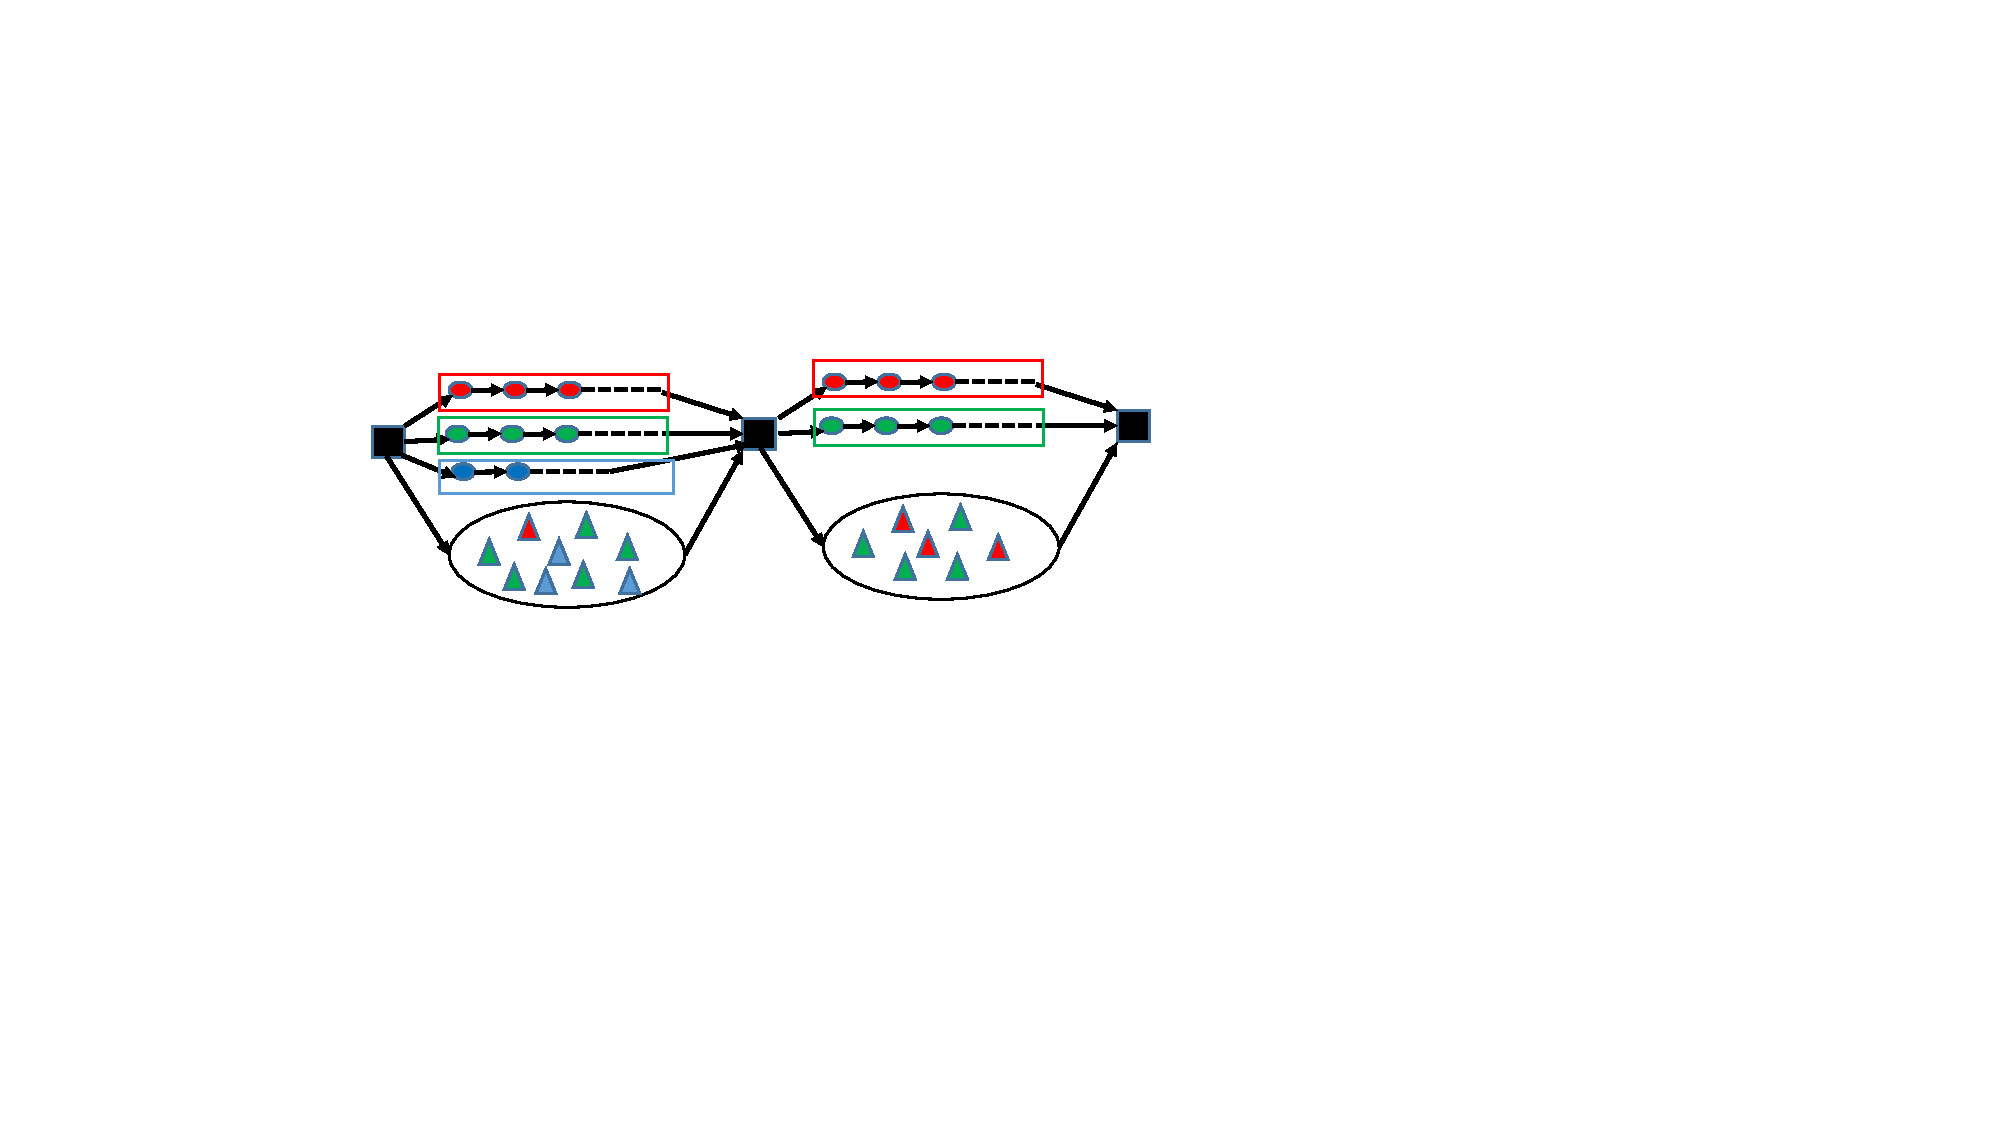
\includegraphics[width=3in]{figures/synchschemas/SPS2.pdf}
  \caption{Illustrative partially ordered stream.}
  \label{fig:ex-postream}
\end{figure}

The idea of this definition is to model partially ordered streams like the one visualized in \Cref{fig:ex-postream}.
This partial order consists of a sequence of black squares $\blacksquare$ with streams in between, which is described by the type $\hier{\blacksquare}{S}$.
The substream type $S$ consists of circles and triangles combined in parallel: $\parcomp{S_1}{S_2}$.
The parallel substream of circles (type $S_1$) consists of a sequences of circles $\bigcirc$, described by $\keyby{K}{\seqleaf{\bigcirc}}$.
The type $K$ in the ParBy construct is a \emph{key} field $K$ that describes the index of the set of substreams (the key on which they are partitioned).
Colors are used to indicate different values of the field $K$
Second, the parallel substream of triangles $\triangle$ is simply a bag, described by $\relleaf{\triangle}$.
Here the colors indicate different values of the base type; note that equal values and unequal values are all parallel in a bag, unlike in ParBy.

Thus, overall, this illustration of a stream is described by the following type:
\[
\hier{\blacksquare}{\parcomp{ \quad \keyby{K}{\seqleaf{\bigcirc}}}{\quad \relleaf{\triangle} \quad}}.
\]

\Cref{45:fig:example-schema} shows this stream type visualized as a tree.
Siblings correspond to the \parcomp{S_1}{S_2} constructor while the rectangular box,
labeled with the key fields, corresponds to the \keyby{K}{S} constructor.
A parent node with several children corresponds to the $\hier{T}{S}$ constructor.

\begin{figure}[t]
  \centering
  \begin{tikzpicture}[sibling distance=11em,
    every node/.style = {shape=rectangle,
      rounded corners,
      draw, align=center}]
    \node { \TopSchemaNode{ $\blacksquare$ }}
      child {
          \SchemaNode{\seqleaf{ \bigcirc }}{s2}
      }
      child {
          \SchemaNode{\relleaf{ \triangle } }{s3}
      };
    \KeyByNode{$K$}{k1}{s2}{s2};
  \end{tikzpicture}
  \caption{Example stream type for \Cref{fig:ex-postream} drawn as a tree.}
  \label{45:fig:example-schema}
\end{figure}

This example is abstracted, but represents a practical use case such as the following example.

\begin{example}
\label{45:ex:taxi-distance-schema-headers}
\label{45:ex:taxi-distance-schema}
Consider a stream of taxi events, where each is a GPS measurement, an indication of a taxi ride begin or a ride end, or an end-of-hour synchronization marker.
GPS data for each taxi is a tuple type $\bigcirc =$ \texttt{GPS(x: float, y: float, z: float)}, which indicates the type of a GPS measurement using three dimensional coordinates.
Completed ride data is a tuple type $\triangle =$ \texttt{RideCompleted(rideID: int, passengerID: int, cost: int)}.
Finally, end-of-hour events are used to synchronize in time; these are a tuple type $\blacksquare =$ \texttt{EndOfHour(date: date, hour: int)}.

The stream shown in \Cref{fig:ex-postream} applies to this example where squares, circles, and triangles are events of the corresponding tuple types as described above.
The relationship between the different tuple types is described by the stream type shown in \Cref{45:fig:example-schema}.
Described from the bottom up: first, the type $S_1 = \keyby{\texttt{taxiID}}{\seqleaf{\texttt{GPS}}}$ denotes that \texttt{GPS} events are partitioned by the key \texttt{TaxiID} and are totally ordered for each taxi.
Second, $S_2 = \relleaf{\texttt{RideCompleted}}$ denotes that \texttt{RideCompleted} events are unordered, and can be considered to be a bag.
Finally, $S = \hier{\texttt{EndOfHour}}{\parcomp{S_1}{S_2}}$ denotes that \texttt{EndOfHour} events synchronize the events in $S_1$ and $S_2$, each of which can be processed in parallel as they are independent.
\end{example}

The partially ordered structures we have in mind (like the illustration of \Cref{fig:ex-postream}) can be viewed in multiple ways, and we explore this formally in the next section.
In particular, we will define what it means for a labeled partially ordered set to be a value of type $S$ for a stream $S$ in \Cref{view:labeled-posets}.

\section{Views of Streams}

\subsection{Streams as Structured Batches}
\label{view:batches}

The following syntax defines concrete \emph{structured} stream instances for each of the
stream types, which we call \emph{batches} because they represent data
collected into a static bundle.\footnote{Thanks to Joe Cutler for this suggestion.}
To define a concrete stream instance, one either defines a pair, a sequence, or a bag (unordered multiset).
\[
  B \quad ::= \quad
    (B, B) \mid
    [B, B, \ldots, B] \mid
    \{B, B, \ldots, B\} \mid
    t: T
\]

Batches are typed using the following typing rules:

\begin{mathpar}
    \inference[Synch]
    {
      t_i: T \\
      \batchtype{b_i}{S}
    }
    {
      \batchtype{[b_0, t_1, b_1, t_2, b_2, \ldots, t_m, b_m]}{\hier{T}{S}}
    }
    \\

    \inference[Par]
    {
      \batchtype{b_1}{S_1} \\
      \batchtype{b_2}{S_2} \\
    }
    {
      \batchtype{(b_1, b_2)}{\parcomp{S_1}{S_2}}
    }

    \\

    \inference[ParBy]
    {
      k_i: K \\
      k_i \ne k_j \text{ for } i \ne j \\
      \batchtype{b_i}{S} \emph{ nonempty}
    }
    {
      \batchtype{\{(k_1, b_1), (k_2, b_2), \ldots, (k_n, b_n)\}}{\keyby{K}{S}}
    }

    \\

    \inference[Bag]
    {
      t_i: T
    }
    {
      \batchtype{\{t_1, t_2, \ldots, t_n\}}{\relleaf{T}}
    }

    \inference[Emp]
    {
      \;
    }
    {
      \batchtype{[]}{\empstream{}}
    }
\end{mathpar}

The \emph{nonempty} requirement in the \textsc{ParBy} case is the inductive property that holds exactly when the batch has no occurences of $t: T$ for any base type $T$.
Specifically, $(b_1, b_2)$ is empty if $b_1$ and $b_2$ are empty;
a list is empty if and only if each of its elements is empty;
and a bag is empty if and only if each of its elements is empty.
The batch $t: T$ is never empty.

\subsection{Stream Events and Dependence Relation}
\label{view:events}

A stream can also be thought of as a type for individual events in isolation.
Events can be either base types or tuples.
Tuples are needed because if $K_1, \ldots, K_n$ are types of keys and $T$ is a payload type,
an event is a tuple of an element of each key and an element of the payload.
Here is a grammar for events:
\[
  E \quad ::= \quad (E, E) \mid t: T
\]

We can also talk about events specific to a particular stream type:
$\eventtype{e}{S}$ means that $e$ is a valid event for a stream type $S$.
Notice that there are no rules for $\eventtype{t}{\empstream{}}$ -- there are no events of the empty stream type.

\begin{mathpar}
    \inference[Synch-1]
    {
      e: T
    }
    {
      \eventtype{e}{\hier{T}{S}}
    }

    \inference[Synch-2]
    {
      \eventtype{e}{S}
    }
    {
      \eventtype{e}{\hier{T}{S}}
    }
    \\

    \inference[Par-1]
    {
      \eventtype{e}{S_1}
    }
    {
      \eventtype{e}{\parcomp{S_1}{S_2}}
    }

    \inference[Par-2]
    {
      \eventtype{e}{S_2}
    }
    {
      \eventtype{e}{\parcomp{S_1}{S_2}}
    }

    \\

    \inference[ParBy]
    {
      k: K \\
      \eventtype{e}{S}
    }
    {
      \eventtype{(k, e)}{\keyby{K}{S}}
    }

    \inference[Bag]
    {
      e: T
    }
    {
      \eventtype{e}{\relleaf{T}}
    }
\end{mathpar}

However, a stream type is more than just its type of events.
In addition, a stream defines a \emph{dependence relation}, a symmetric binary relation
on pairs of events.
The relation indicates whether the events should be considered ordered with respect to each other.
For example, in \Cref{fig:ex-postream}, red circles are dependent with each other but independent of green circles;
all circles are dependent with black squares.
One quirk of this model is that because partial orders are transitive,
red circles in on the left are ordered with green circles on the right,
though they are not dependent;
so the dependence relation indicates forced orderings, but additional
orderings may be derived by transitivity.

The dependence relation
$\deptype{e}{e'}{S}$ means that events $e$ and $e'$ are dependent
with respect to the stream tyep $S$ (the events should in particular satisfy $\eventtype{e, e'}{S}$).
This is defined by the following rules.
Notice that there are no rules for
$\empstream{}$ (because it has no events)
nor for $\relleaf{}$ (because all events in a bag are independent).

\begin{mathpar}
    \inference[Synch]
    {
      t: T \\
      \eventtype{e}{\hier{T}{S}}
    }
    {
      \deptype{e}{t}{\hier{T}{S}} \\
      \deptype{t}{e}{\hier{T}{S}}
    }

    \inference[Sub]
    {
      \deptype{e}{e'}{S}
    }
    {
      \deptype{e}{e'}{\hier{T}{S}}
    }
    \\

    \inference[Par-1]
    {
      \deptype{e}{e'}{S_1}
    }
    {
      \deptype{e}{e'}{\parcomp{S_1}{S_2}}
    }

    \inference[Par-2]
    {
      \deptype{e}{e'}{S_2}
    }
    {
      \deptype{e}{e'}{\parcomp{S_1}{S_2}}
    }
    \\

    \inference[ParBy]
    {
      k: K \\
      \deptype{e}{e'}{S}
    }
    {
      \deptype{(k, e)}{(k, e')}{\keyby{K}{S}}
    }
\end{mathpar}

Inductively, $\deptype{e}{e'}{S}$ is the smallest relation defined by the above rules.
It is symmetric, i.e. $\deptype{e}{e'}{S}$ iff $\deptype{e'}{e}{S}$ by an easy induction on the typing judgment.
If two events $\eventtype{e, e'}{S}$ are \emph{not} dependent, we say they are independent and write
$\indeptype{e}{e'}{S}$.
Dependence is constructive and decidable via the above rules, so we could have alternatively given a typing judgment for $\indeptype{e}{e'}{S}$.
For completeness, such a typing judgment is shown in \Cref{omitted:typing}.

We also could have given both $\deptype{e}{e'}{S}$ and $\indeptype{e}{e'}{S}$ as a single Boolean-valued function on pairs of events,
i.e. $\event{S} \times \event{S} \to \texttt{bool}$.

\subsection{Stream Linearizations and Equivalence Relation}
\label{view:linearizations}

A \emph{linearization} is a sequence of events:
\[
  L \quad ::= \quad [E, E, \ldots, E]
\]
Notice that each event in the sequence may be different (they may even all have different types).
Linearizations support the operations of concatenation ($\cdot$), the interleaving relation
$\lininterleave{l}{l_1, l_2, \ldots, l_k}$,
meaning that $l$ consists of $l_1, l_2, \ldots, l_k$ interleaved in some order.
% and the element-wise product: for $t: E$ and $e_i: E$,
% \[
%   t \times [e_1, e_2, \ldots, e_n] := [(t, e_1), (t, e_2), \ldots, (t, e_n).
% \]

Linearizations are typed using the rule that \emph{a linearization has type $S$ if all its elements are events of $S$}:
\begin{mathpar}
    \inference[Lin]
    {
      l = [e_1, e_2, \ldots, e_n] \\
      \eventtype{e_i}{S} \text{ for all } i
    }
    {
      \lintype{l}{S}
    }

    % \inference[Synch]
    % {
    %   t_i: T \\
    %   \lintype{l_i}{S} \\
    %   l = l_0 \cdot [t_1] \cdot l_1 \cdot [t_2] \cdots [t_m] \cdot l_m
    % }
    % {
    %   \lintype{l}{\hier{T}{S}}
    % }
    %
    % \\
    %
    % \inference[ParBy]
    % {
    %   k_i: T \\
    %   \lintype{l_i}{S} \\
    %   l_i \ne [] \\
    %   \lininterleave{l}{k_1 \times l_1, k_2 \times l_2, \ldots, k_n \times l_n}
    % }
    % {
    %   \lintype{l}{\keyby{T}{S}}
    % }
    %
    % \\
    %
    % \inference[Par]
    % {
    %   \lininterleave{l}{l_1, l_2} \\
    %   \lintype{l_1}{S_1} \\
    %   \lintype{l_2}{S_2} \\
    % }
    % {
    %   \lintype{l}{\parcomp{S_1}{S_2}}
    % }
    %
    % \\
    %
    % \inference[Bag]
    % {
    %   t_i: T
    % }
    % {
    %   \lintype{[t_1, t_2, \ldots, t_n]}{\relleaf{T}}
    % }
    %
    % \inference[Emp]
    % {
    %   \;
    % }
    % {
    %   \lintype{[]}{\empstream{}}
    % }
\end{mathpar}

% No longer needed
% \begin{proposition}
% \label{prop:lin-event-correspondence}
% \begin{enumerate}
% \item Linearizations are the same as sequences of events:
% for any stream type $S$ and sequence $l = [e_1, e_2, \ldots, e_n]$,
% \[
% \lintype{l}{S} \quad \text{iff} \quad \eventtype{e_i}{S} \text{ for all } i.
% \]
% \end{enumerate}
% \end{proposition}
% \begin{proof}
% \end{proof}

The dependence relation also gives rise to an equivalence relation on linearizations.
This equivalence relation is derived as follows:

\begin{mathpar}
    \inference[Indep]
    {
      \indeptype{e}{e'}{S}
    }
    {
      \equivtype{[e, e']}{[e', e]}{S}
    }

    \inference[Concat]
    {
      \equivtype{l_1}{l_1'}{S} \\
      \equivtype{l_2}{l_2'}{S}
    }
    {
      \equivtype{l_1 \cdot l_2}{l_1' \cdot l_2'}{S}
    }

    \\

    \inference[Refl]
    {
      \lintype{l}{S}
    }
    {
      \equivtype{l}{l}{S}
    }

    \inference[Trans]
    {
      \equivtype{l}{l'}{S} \\
      \equivtype{l'}{l''}{S}
    }
    {
      \equivtype{l}{l''}{S}
    }
\end{mathpar}

We should immediately check that equivalence respects our typing judgment (i.e., equivalence is only defined between well-typed linearizations):
\begin{proposition}
\label{prop:equiv-preserves-typing}
If $\equivtype{l}{l'}{S}$ then $\lintype{l}{S}$ and $\lintype{l'}{S}$.
\end{proposition}
\begin{proof}
By induction on the typing judgment for $\equivtype{l}{l'}{S}$.
The base case \textsc{Refl} and inductive case \textsc{Trans} are immediate.
For the base case \textsc{Indep}, the independence precondition is only defined for events $\eventtype{e, e'}{S}$.
Finally for \textsc{Concat}, we observe that linearizations of type $S$ are closed under concatenation by the definition \textsc{Lin} of $\lintype{l}{S}$,
since it states a condition on each element of the sequence individually.
\end{proof}

The other important thing to check immediately is that concatenation respects equivalence, but we don't need to prove this as this is baked into the definition: in particular, the \textsc{Concat} rule forces this. It says that equivalent linearizations concatenate to get equivalent linearizations.

\subsection{Streams as Labeled Posets}
\label{view:labeled-posets}

For our last view of a streams, we define the concept of \emph{labeled poset}, which we also may abbreviate as \emph{polset} (for partially ordered, labeled set). This concept is traditionally called a \emph{pomset}, for partially ordered multiset; however, this terminology can be confusing, because the labeling is on the underlying set, not on the elements of the multiset.

A \emph{partially ordered set} $(s, \le)$ is a set $s$ together with a binary relation $\le$ on pairs of elements of $s$ that is reflexive, transitive, and antisymmetric.
A \emph{labeled poset (polset)} of type $X$ is a
partially ordered set $(s, \le)$ together with a labeling function $\ell: s \to X$.
We denote this $(s, \le, \ell)$. A labeled poset is different than a poset over $X$ because multiple elements may be labeled with the same element of $X$.
Two posets are \emph{equivalent} if the posets are isomorphic and the isomorphism exactly preserves the labeling $\ell$.

Then we can finally define the last view of streams, as partially ordered sets.
We write
\[
\posettype{(s, \le, \ell)}{S}
\]
if $\ell: s \to \event{S}$ such that the order is consistent with the dependence
relation in the following way:
\begin{enumerate}
\item[(i)] If $\deptype{\ell(i)}{\ell(j)}{S}$ then $i \le j$ or $j \le i$; and
\item[(ii)] No relaxation of $\le$ satisfies (i).
\end{enumerate}

\section{Examples}

We illustrate the different views of streams with the simplest example of values and barriers from \Cref{ex:value-barrier}. The stream type corresponding to this example is
\[
S = \hier{\#}{\relleaf{\texttt{int}}}
\]
where $\#$ denotes a barrier and \texttt{int} denotes a value (integer).
Intuitively, this creates a stream of integers in parallel synchronized by $\#$ markers.
The stream views for this example are as follows:
\begin{itemize}
\item A \emph{batch} of type $S$ in this case is an odd-length list, where every other element is a barrier event. For example:
\begin{align*}
  \batchtype{[\{\}]}{S}& \\
  \batchtype{[\{1, 1, 2\}]}{S}& \\
  \batchtype{[\{1\}, \#, \{2\}]}{S}& \\
  \batchtype{[\{1\}, \#, \{1, 1, 2\}, \#, \{\}]}{S}&
\end{align*}
\item An \emph{event} of type $S$ is either a value or a barrier. Anything is dependent with barrier, but values are not dependent with each other. For example:
\begin{align*}
  \eventtype{1}{S}& \\
  \eventtype{2}{S}& \\
  \eventtype{\#}{S}& \\
  \deptype{1}{\#}{S}& \\
  \deptype{\#}{\#}{S}& \\
  \indeptype{1}{2}{S}&
\end{align*}
\item A \emph{linearization} of type $S$ is a sequence of values and barriers. Two linearizations are equivalent ($\equiv$) mod $S$ if they are the same up to reordering values between adjacent barriers. For example:
\begin{align*}
  \lintype{[]}{S}& \\
  \lintype{[1, 3, 2, 1]}{S}& \\
  \lintype{[1, \#, 2, \#, 3]}{S}& \\
  \lintype{[1, \#, \#, \#, 2, 1]}{S}& \\
  \equivtype{[1, 2]}{[2, 1]}{S}& \\
  \equivtype{[\#, 1, 3, 2, 1, \#]}{[\#, 1, 1, 2, 3, \#]}{S}& \\
\end{align*}
We would \emph{not}, however, have equivalence between $[1, \#]$ and $[\#, 1]$, since $1$ and $\#$ are dependent (don't commute).
\item Finally, a \emph{partial order} of type $S$ consists of a partially ordered set labeled with values and barriers in a consistent way:
\[
\begin{tikzpicture}
  \matrix (m) [matrix of math nodes, column sep=3em, row sep=0.5em]
  {
            &          & |(a3)|1 &          \\
    |(a1)|1 &          &         &          \\
            & |(b1)|\# & |(a4)|2 & |(b2)|\# \\
    |(a2)|3 &          &         &          \\
            &          & |(a5)|1 &          \\
  };
  \path[->]
    (a1) edge (b1)
    (a2) edge (b1)
    (b1) edge (a3) edge (a4) edge (a5)
    (a3) edge (b2)
    (a4) edge (b2)
    (a5) edge (b2);
\end{tikzpicture}
\]
Notice that the barrier $\#$ events are ordered with everything, and the value events are unordered as much as possible (except for their order with $\#$).
Since partial orders are transitive, this also implies some orderings on values; for example, the $1$ and $3$ in the first column are ordered less than the $1, 2, 1$ in the third column.

\end{itemize}

\section{Isomorphism between Views}
\label{sec:isomorphism-between-views}

\subsection{Isomorphism between Batches and Linearizations}

\begin{definition}[Flattening]
    \label{def:batch-flattening}
    Let $S$ be a stream type,
    and let $\batchtype{b}{S}$.
    A \emph{flattening} $l$ of $b$ is any linearization
    defined inductively on $S$ as follows:
\begin{itemize}
\item If $S = \empstream{}$, then $b = []$ and $l$ is a flattening of $b$ if and only if $l = []$.
\item If $S = \relleaf{\mathcal{H}}$, then $b$ is a multiset, and $l$ is a flattening of $b$ if and only if the multiset of events in $l$ equals $b$.
(That is, $l$ contains exactly the same events as $b$ in some order. Assuming $b$ has at least two distinct elements, there will be multiple such flattenings.)
\item In case $S = \hier{T}{S'}$, we have $b = [b_0, t_1, b_1, t_2, b_2, \cdots, t_m, b_m]$ for some batches $\batchtype{b_i}{S'}$.
Then $l$ is a flattening of $b$ if and only if $l = l_0 \cdot [t_1] \cdot l_1 \cdot [t_2] \cdot l_2 \cdot \ldots \cdot [t_m] \cdot l_m$,
where $l_i$ is a flattening of $b_i$ for all $i$.
\item In case $S = \parcomp{S_1}{S_2}$, we have $b = (b_1, b_2)$.
Then $l$ is a flattening of $b$ if and only if $l$ is an interleaving of some $l_1, l_2$ where $l_1$ is a flattening of $b_1$ and $l_2$ is a flattenign of $b_2$.
That is, $\lininterleave{l}{l_1, l_2}$.
\item Finally, in case $S = \keyby{K}{S'}$, we have $b$ is a set with finitely many entries $(v_i, b_i)$ for $i = 1, \ldots, m$.
Then $l$ is a flattening of $b$ if and only if $l$ is an interleaving of the sequences $l_1, l_2, \ldots, l_m$
where $l_i$ is a flattening of $t_i$ for each $i$.
That is, $\lininterleave{l}{l_1, l_2, \ldots, l_m}$.
\end{itemize}
\end{definition}

\begin{proposition}
\label{prop:batch-lin-correspondence}
Let $S$ be a stream type such that all base types in $S$ are unique.
\begin{enumerate}
\item[(1)] For every linearization $\lintype{l}{S}$, there exists a \emph{unique} batch $b$ such that $\batchtype{b}{S}$ and $l$ is a flattening of $b$. Call this batch $b = \parselin{l}{S}$.
\item[(2)] For every batch $\batchtype{b}{S}$, every flattening $l$ of $b$ satisfies $\lintype{l}{S}$.
\item[(3)] For every batch $\batchtype{b}{S}$, there exists at least one flattening $l$ of $b$.
\item[(4)] For two linearizations $\lintype{l_1, l_2}{S}$ we have $\equivtype{l_1}{l_2}{S}$ if and only if $\parselin{l_1}{S} = \parselin{l_2}{S}$
\item[(5)] Finally, if $\batchtype{b}{S}$, then for any two flattenings $l_1, l_2$ of $b$, $\equivtype{l_1}{l_2}{S}$.
\end{enumerate}
\end{proposition}
\begin{proof}
Adapted from Appendix B of~\citeMain{pods21} (Proof of Proposition 14).
By induction on $S$.
For $\relleaf{T}$,
all five conditions state a standard correspondence between a multiset of items and its linearizations.
For $\parcomp{S_1}{S_2}$
and for $\keyby{K}{S_1}$,
we observe that sequences over events $\eventtype{e}{S}$ are interleavings of events each from a subtype,
and all such interleavings are equivalent with respect to $\equiv$, by the rule \textsc{Indep}.
Conversely $\equiv$ only holds between different interleavings of the same two or more sequences up to equivalence, i.e. for parallel composition, if $l \equiv l'$ and $l$ is an interleaving of $l_1$ and $l_2$ and $l_1'$ is an interleaving of $l_2'$, then $l_1 \equiv l_1'$ and $l_2 \equiv l_2'$.
This uses the fact that all base types are unique and can be proven inductively on $\equivtype{l}{l'}{S}$.

The most interesting case is $S = \hier{T}{S'}$.
Here, we essentially apply the idea that $(a \cup b)^{*} = (a^{*} b)^{*} a^{*}$ for languages: in this context $a$ is the type $\event{S'}$ and $b$ is the type $T$.
So a sequence of $\event{S}$ decomposes into a sequence of subsequences over $S'$ delineated by $T$ events, where there is one more subsequence than the number of $T$ events.
Since $T$ events are fully dependent on everything else (rule \textsc{Synch}), this decomposition is not changed by $\equiv$, which can thus be identified with equality on the sequence of $T$ events together with equivalence on each $\event{S'}$ substream.
The definition of flattening reflects this decomposition exactly.
\end{proof}

It is worth noting that \emph{not all} binary relations on pairs of $\event{S}$ arise as a dependence relation $\deptype{e}{e'}{S}$.
In particular, the (symmetric reflexive closure of)
the relations $\{(A, B), (B, C), (C, D)\}$
and $\{(A, B), (B, C), (C, D), (D, A)\}$
do not have a hierarchical structure:
here there is no way to choose a header out of $A, B, C, D$
to be a root node in the stream type.

The following proposition
characterizes exactly the dependence relations arising from stream types, based on these two examples.
\begin{proposition}
\label{prop:stream-types-less-general}
For any stream type $S$, the relation $\mathcal{D}$ ($\deptype{e}{e'}{S}$) is symmetric and reflexive.
It additionally satisfies the following restriction:
$\mathcal{D}$ does not contain the cycle graph $C_4 = \{(A, B), (B, C), (C, D)\}$
or the path graph $P_4 = \{(A, B), (B, C), (C, D), (D, A)\}$ when restricted
to any set of four base types $a, b, c, d$.
\end{proposition}
\begin{proof}
Symmetry and reflexivity are by construction in each type constructor for
$\mathcal{D}$.

Now suppose that we introduce a cycle $C_4$ or path $P_4$.
It cannot have been introduced in the base case $\relleaf{T}$,
% or $\seqleaf{T}$,
nor in parallel composition since $C_4$ and $P_4$ are connected;
nor in $\keyby{K}{S}$ since there are no dependencies across keys.
So it must have been introduced by the $\hier{T}{S}$ construct.
But for either $C_4$ or $P_4$, there is no way to partition (cut) the vertices into those in
$T$ and those in $S$ (with at least one vertex in each partition) such that every event in the first is
dependent on every event in the second.
\end{proof}

\subsection{Concatenation on Batches}

Because batches are isomorphic to linearizations up to equivalence (as just shown in \Cref{prop:batch-lin-correspondence}), we can define concatenation on batches. In particular, if $l_1$ and $l_2$ are linearizations of type $S$,
their concatenation $l = l_1 \cdot l_2$ is a linearization of type $S$,
so it has a unique parsing $\batchtype{\parselin{l}{S}}{S}$.
To show that this lifts to an operation on batches $b_1 \circ b_2$, it remains to show that this is well-defined up to equivalence on linearizations:
\begin{proposition}
\label{batch-concatenation-well-defined}
Batch concatenation $b_1 \circ b_2$ is well-defined and associative: $(b_1 \circ b_2) \circ b_3 = b_1 \circ (b_2 \circ b_3)$.
\end{proposition}
\begin{proof}
By the \textsc{Concat} rule as remarked earlier, $\equivtype{l_1}{l_1'}{S}$ and $\equivtype{l_2}{l_2'}{S}$
then $\equivtype{l_1 \cdot l_2}{l_1' \cdot l_2'}{S}$.
Then consider flattenings $l_1$ and $l_2$ of $b_1$ and $b_2$ respectively;
by \Cref{prop:batch-lin-correspondence} (3), (5),
$l_1$ and $l_2$ are unique up to equivalence;
by the \textsc{Concat} rule the concatenation $l_1 \cdot l_2$ is unique up to equivalence;
and by \Cref{prop:batch-lin-correspondence} (4)
this means $\parselin{l_1 \cdot l_2}{S}$ is the same regardless of the choice of $l_1$ and $l_2$.

Associativity follows by associativity of concatenation on sequences since concatenation respects equivalence.
\end{proof}

\subsection{Isomorphism between Linearizations and Labeled Posets}

Given any stream type $S$, any linearization $\lintype{l}{S}$ gives rise to a labeled poset, which we call $\posetlin{l}{S}$ as follows:
if $l$ has length $n$, then we let $s = \{1, 2, \ldots, n\}$, and we define the labeling function $\ell(i) = l[i]$.
Then we define the ordering as follows:
$i <_{l, S} j$ iff there is some sequence of indices
\[
i = i_0 < i_1 < \ldots < i_m = j
\]
such that each pair adjacent in the sequence is dependent:
\[
\deptype{l[i_0]}{l[i_1]}{S}, \deptype{l[i_1]}{l[i_2]}{S}, \ldots, \deptype{l[i_{m-1}]}{l[i_m]}{S}.
\]

This definition may look opaque, but captures the property that $l[i]$ and $l[j]$ are ordered: it is impossible to reorder them to get $l[j]$ before $l[i]$.
The following proposition justifies this formally:
\begin{proposition}
\label{prop:lin-poset-correspondence}
Let $S$ be a stream type such that all base types in $S$ are unique.
\begin{enumerate}
\item[(1)] Let $\lintype{l_1}{S}$ and $\lintype{l_2}{S}$ be two linearizations.
Then $\equivtype{l_1}{l_2}{S}$ if and only if $\posetlin{l_1}{S_1}$ and $\posetlin{l_2}{S_2}$ are isomorphic.
\item[(2)] Let $\lintype{l}{S}$ be a linearization; then $\posettype{\posetlin{l}{S}}{S}$.
\item[(3)] Let $\posettype{p}{S}$; then there exists a linearization $l$ such that $p$ is isomorphic to $\posetlin{l}{S}$.
\end{enumerate}
\end{proposition}
\begin{proof}
For (1) in the forward direction, what we need to show is that the rules for $\equiv$ preserve poset isomorphism. For the rule \textsc{Indep} the isomorphism switches $e$ and $e'$ in the linearization; this preserves the order because $e$ and $e'$ are not ordered under $<_{l, S}$. \textsc{Refl} and \textsc{Trans} hold because poset isomorphism is transitive. Finally for \textsc{Concat}, we construct an isomorphism between the posets on $l_1 \cdot l_2$ and $l_1' \cdot l_2'$ by combining the isomorphisms on the first half and second half. The idea is then that any ordering in $<_{l_1 \cdot l_2, S}$ defined by $i = i_0 < i_1 < \ldots < i_m = j$ is derived from a first half of orderings in $l_1$, followed by a second half of orderings in $l_2$,
which is isomorphic to a segment of orderings in $l_1'$ followed by a segment of orderings in $l_2'$, which implies ordering in $<_{l_1' \cdot l_2', S}$.
The reverse direction requires decomposing any isomorphism by induction into a matching between the elements of the individual linearizations such that the matchign can be formed by repeated consecutive swaps, implying equivalence via \textsc{Indep}, \textsc{Concat}, and \textsc{Trans}; this is the same as for data-trace types and a full proof can be found in~\citeMain{pldi19} and~\citeMain{festschrift18}.

For (2), the crux of the statement is that our definition of $<_{l, S}$ precisely captures the smallest ordering consistent with dependence $\mathcal{D}$ as described in the definition of a poset. Since $\deptype{l[i]}{l[j]}{S}$ implies that $i <_{l, S} j$ or vice versa, $<_{l, S}$ is an ordering consistent with $\mathcal{D}$, so it remains to see why there is no weaker ordering. But note that any weaker ordering would have to remove $i <_{l, S} j$ for some $i < j$ as these are the atomic constraints generating the ordering, and then it would not be consistent with $\mathcal{D}$.

Finally, for (3), for an arbitrary finite labeled poset $p$ of size $n$ pick any topological ordering of its elements $1, 2, 3, \ldots, n$, and consider the linerization $\lintype{l}{S}$ defined by elements $1, 2, 3, \ldots, n$ in that order. The ordering arising from $p$ must contain all pairs $i <_{l, S} j$ where $\deptype{l[i]}{l[j]}$ because otherwise $i$ and $j$ would be indepdent, violating consistency with $\mathcal{D}$; and it must be the smallest ordering containing these pairs by minimality of $p$.
\end{proof}

\section{Stream Type Relaxation}

We define relaxation, a form of semantic subtyping: $S_1$ is a relaxation of $S_2$ means that a stream of type $S_2$ can be interpreted as a stream of type $S_1$ if the partial order is relaxed.
The following are adapted from Section 2.5 and Appendix B of~\citeMain{pods21}.
We assume some subtyping relation on base types, which can be trivial if unwanted;
in that case the relaxation requires type equality $\event{S_1} = \event{S_2}$.

\begin{definition}[Stream relaxation]
\label{def:stream-relaxation}
For stream types $S_1$ and $S_2$,
$S_1$ is a \emph{relaxation} of $S_2$, written $S_1 \lesssim S_2$, if
(i) $\event{S_1}$ is a supertype of $\event{S_2}$
and (ii) for all tuples $\eventtype{x, y}{S_2}$,
if $\deptype{x}{y}{S_1}$ then $\deptype{x}{y}{S_2}$.

Two stream types $S_1$ and $S_2$ are \emph{order-equivalent}, denoted $S_1 \sim S_2$, if both $S_1 \lesssim S_2$ and $S_2 \lesssim S_1$.
\end{definition}

\begin{proposition}
\label{prop:stream-relaxation-lin}
\label{45:prop:schema-relaxation-flattening}
Suppose that $S' \lesssim S$. Then:
(1) If $\lintype{l}{S}$ then $\lintype{l}{S'}$.
(2) If $\equivtype{l_1}{l_2}{S}$ then $\equivtype{l_1}{l_2}{S'}$.
\end{proposition}
\begin{proof}
Statement (1) is direct from the fact that $\event{S'}$ is a supertype of $\event{S}$
and linearizations are sequences of events.
For (2) all typing rules for $\equivtype{l_1}{l_2}{S'}$ are the same as for $\equivtype{l_1}{l_2}{S}$ except \textsc{Indep}, which introduces strictly more equivalences by condition (ii) of the relaxation.
\end{proof}
% Proof of similar fact for synch schemas but stated in terms of flattenings:
%
% We first show uniqueness. Let $t_1', t_2': S'$
% such that every flattening of $t$ is a flattening of $t_1'$ and of $t_2'$.
% Since every SPS has at least one flattening,
% we can choose some particular flattening $s$ of $t$
% (a sequence over $\headers(S)$).
% By uniqueness in Proposition~\ref{45:prop:sps-sequence-correspondence}-(1),
% since $s$ is a flattening of both $t_1'$ and $t_2'$, $t_1' = t_2'$.
%
% Now we show existence.
% As before, choose a particular flattening $s$ of $t$.
% Since $\headers(S') \supseteq \headers(S)$,
% $s$ is also a sequence over $\headers(S')$.
% Thus by Proposition~\ref{45:prop:sps-sequence-correspondence}-(1),
% there exists a $t': S'$ such that $s$ is a flattening
% of $s$.
% It remains to show that all flattenings of $t$ are flattenings of $t'$.
% Given any flattening $\hat{s}$ of $t$,
% by Proposition~\ref{45:prop:sps-sequence-correspondence}-(2b),
% $s \equiv_{D_{S}} \hat{s}$.
% By the definition of relaxation,
% $s \equiv_{D_{S'}} \hat{s}$.
% Then by Proposition~\ref{45:prop:sps-sequence-correspondence}-(2a),
% $\hat{s}$ is a flattening of $t'$.

\begin{theorem}
\label{thm:stream-relaxation-decidable}
Stream relaxation, that is on input two stream types $S_1$ and $S_2$, checking if $S_1 \lesssim S_2$ (and consequently checking stream type equivalence), is decidable in quadratic time.
\end{theorem}
\begin{proof}
We may ignore the base types in $S_1$ and not in $S_2$.
Then for each pair of base types $T, T'$ in $\event{S_2}$,
we build a formula $\phi^1_{T, T'}$ whose free variables are elements of $T$ and elements of $T'$ or fields of $T$ and fields of $T'$ in case they are tuple types,
which is true exactly when
$\deptype{x}{x'}{S_1}$ for $x : T$ and $x' : T'$.
This is done by expanding out the cases for the dependence relation $D$.
In all case the formula built is either true or false, or a derived from a subcase,
except in the $\keyby{K}{S}$ case where
we get an equality constraint as an atomic formula:
specifically, for $\deptype{(k, e)}{(k', e')}{\keyby{K}{S}}$
we get the constraint $k = k'$ (in conjunction with the recursive formula for $\deptype{e}{S}{S'}$).
Altogether, each $\phi^1_{T, T'}$ is just an atomic formula over the
language of equality.
We do the same for $S_2$ to get formulas $\phi^2_{T, T'}$.

The problem now becomes checking a set of implications
of atomic formulas over the language of equality, which is
decidable by checking each implication
$\phi^1_{T, T'} \to \phi^2_{T, T'}$
in turn.
The complexity is quadratic because there are quadratically many pairs $T, T'$.
\end{proof}

\section{Monotonicity, Type Safety, and Determinism}
\label{sec:operator-properties}

Finally, we define three key properties that are relevant to the rest of the thesis: monotonicity, type safety, and determinism for operators over streams.
First, we need an abstract model of an operator in a stream processing system.
\begin{definition}
\label{def:operator}
An \emph{operator} from type $X$ to type $Y$ is a relation
$F \subseteq \listtype{X} \times \listtype{Y}$ such that each input is associated with at least one output:
for every $l: \listtype{X}$, there exists $l': \listtype{Y}$
such that $(l, l') \in F$.
\end{definition}

Modeling the operator as a relation is necessary because it allows for nondeterministic behavior; that is, this is a model of a concurrent system with multiple possible execution traces. The definition only requires that there is at least one possible behavior on any given input stream.

A bit of foreshadowing: though they aren't directly expressed as such, operators are basically the key objects studied in \Cref{cha:distribution,cha:testing,cha:monitoring}.
\Cref{cha:composition} is not quite eligible for this distinction as it only defines functions on batches, but these can also be seen as operators by applying our isomorphism from \Cref{sec:isomorphism-between-views}; see \Cref{thm:type-safe-and-deterministic-converse}.

For the following properties, let $S$ be an input stream type, $S'$ an output stream type, and $F$ an operator from $\event{S}$ to $\event{S'}$.
\begin{itemize}
  \item \textbf{Monotonicity:} $F$ is \emph{monotone}
  if for all $(l, l') \in F$, if $l$ is a prefix of $m$, then there
  exists $m'$ such that $l'$ is a prefix of $m'$ and $(m, m') \in F$.

  \item \textbf{Type safety:} $F$ is \emph{type safe} if, for all $(l_1, l_1') \in F$ and $\equivtype{l_1}{l_2}{S}$ there exists $l_2'$ such that $\equivtype{l_1'}{l_2'}{S'}$ and $(l_2, l_2') \in F$.

  \item \textbf{Determinism:} $F$ is \emph{deterministic up to output equivalence}, or simply \emph{deterministic}, if whenever $(l, l_1') \in F$ and $(l, l_2') \in F$, $\equivtype{l_1'}{l_2'}{S'}$.
\end{itemize}

\subsection{Examples}

To illustrate monotonicity, consider the function \textsc{Sum} (encoded as an operator as a set of ordered pairs), which takes in a sequence or bag of integers and outputs their sum.
The input stream type is \seqint{} (\relint{} also works)
and the output type is \seqint{} (though there is only be one output, so it is really a singleton).
\textsc{Sum} is not monotonic because on input $[1, 2, 3]$ it produces $[6]$ and on input $[1, 2, 3, 1]$ it produces $[7]$, but $[6]$ is not a prefix of $[7]$. To make it monotonic, we have to add an special sharp symbol to trigger output: the correct function to consider is the one which maps $[1, 2, 3]$ to $[]$, but maps $[1, 2, 3, \#]$ to $6$.
Specifically, we define \textsc{SumAt} which maps
maps $[a_1, a_2, a_3, \ldots, a_k, \#] + t$ to $[a_1 + a_2 + \cdots + a_k]$ for any integers $a_1, \ldots, a_k$ and any tail list $t$, but maps input lists with no instance of $\#$ to $[]$.
We could also choose to trigger output on every $\#$, not just the first one.
Either way, this function is monotonic.
The function \textsc{SumAt} is best described using the input type \synchrelint{} (a sequence of bags separated by $\#$), but could also be described as a simple sequence \seqint{}. Its output type is \seqint{}.

To illustrate type safety, consider the function \textsc{Iden}, which consists of all pairs $(l, l)$, e.g. it maps $[1, 2, 3]$ to $[1, 2, 3]$.
Suppose $S = \relint{}$ so that it allows input reorderings, that is $\equivtype{[1, 2, 3]}{[1, 3, 2]}{S}$.
Then type safety says that there should be an output on $[1, 3, 2]$ that is equivalent to $[1, 2, 3]$ under $S'$.
This holds if, and only if, $\equivtype{[1, 2, 3]}{[1, 3, 2]}{S'}$.
So this identity operator is type safe if and only if $S'$ allows output reorderings.
In particular, it is type safe for $S' = \relint{}$ but \emph{not} for $S' = \seqint{}$.
If instead $S = \seqint{}$, it is type safe either way.

To illustrate determinism, it is immediate that \textsc{Sum} and \textsc{Iden} are deterministic because they are functions. But for a less trivial example, consider the relation \textsc{Forget}, which maps a list $l$ to all its possible reorderings: in particular, for $l = [1, 2, 3]$, \textsc{Forget} contains all six pairs
\[
(l, l), (l, [1, 3, 2]), (l, [2, 1, 3]), (l, [2, 3, 1]), (l, [3, 1, 2]), (l, [3, 2, 1]).
\]
Then \textsc{Forget} is deterministic if, and only if, $\equivtype{l_1}{l_2}{S'}$ for all reorderings (permutations) $l_1$ and $l_2$.
Concretely, it is deterministic for output type $S' = \relint{}$ but not for output type $S' = \seqint{}$.
In short, determinism allows for multiple outputs as long as those outputs are equivalent.

\begin{figure}
\centering
\footnotesize
\renewcommand{\arraystretch}{2.5}
\setlength{\tabcolsep}{3pt}
\begin{tabular}{ccccccc}
  Name & Example I/O & Input type $S$ & Output type $S'$ & Monotone? & Type safe? & Deterministic? \\
  \textsc{Sum}
    & $[1, 2, 3] \mapsto [6]$
    & \seqorrel{} & \seqint{} & \No{} & \Yes{} & \Yes{} \\
  \textsc{SumAt}
    & \makecell{$[1, 2, 3] \mapsto []$ \\ $[1, 2, 3, \#] \mapsto [6]$}
    & \synchrelint{} & \seqint{} & \Yes{} & \Yes{} & \Yes{} \\
  \textsc{Iden}
    & $[1, 2, 3] \mapsto [1, 2, 3]$
    & \seqint{} & \seqorrel{} & \Yes{} & \Yes{} & \Yes{} \\
    && \relint{} & \seqint{} & \Yes{} & \No{} & \Yes{} \\
    && \relint{} & \relint{} & \Yes{} & \Yes{} & \Yes{} \\
  \textsc{Forget}
    & \makecell{$[1, 2, 3] \mapsto [3, 1, 2]$ \\ $[1, 2, 3] \mapsto [1, 2, 3]$}
    & \seqorrel{} & \seqint{} & \Yes{} & \Yes{} & \No{} \\
    && \seqorrel{} & \relint{} & \Yes{} & \Yes{} & \Yes{} \\
  \textsc{First}
    & \makecell{$[1, 2, 3] \mapsto [1]$ \\ $[] \mapsto []$}
    & \seqint{} & \seqorrel{} & \Yes{} & \Yes{} & \Yes{} \\
    && \relint{} & \seqorrel{} & \Yes{} & \No{} & \Yes{} \\
  \textsc{Drop}
    & \makecell{$[1, 2, 3] \mapsto [1, 3]$ \\ $[1, 2, 3] \mapsto [2]$}
    & \seqint{} & \seqorrel{} & \Yes{} & \Yes{} & \No{} \\
    && \relint{} & \seqint{} & \Yes{} & \No{} & \No{} \\
    && \relint{} & \relint{} & \Yes{} & \Yes{} & \No{} \\
\end{tabular}

\caption[Monotonicity, type safety, and determinism examples.]{Examples of monotonicity, type safety, and determinism for a selection of stream operators and input and output types.}
\label{fig:operator-properties-examples}
\end{figure}

It is possible for an operator to be type safe, but not deterministic. For example, if $S' = \seqint{}$, then \textsc{Forget} is not deterministic, but it \emph{is} still type safe because the output, while a set of inequivalent possibilities and not just one, doesn't depend on the input.

It is also possible for an operator to be deterministic, but not type safe.
For example, consider the first-element function \textsc{First} that on $[1, 2, 3]$ returns $[1]$ and on $[2, 1, 3]$ returns $[2]$. This is deterministic because it is a function, whether the input type $S$ is \seqint{} or \relint{}. But if we have $S = \relint{}$, so that $\equivtype{[1, 2, 3]}{[2, 1, 3]}{S}$, then it is not type safe, because $[1]$ and $[2]$ are not equivalent outputs (not even as bags).

Finally, it is possible to be neither deterministic nor type safe.
An interesting example is \textsc{Drop}, which takes the input sequence $l$ and nondeterministically drops some number of items. Formally, $(l, l') \in F$ if $l'$ is any subsequence of $l$. For the types $S = \relint{}$ and $S' = \seqint{}$, \textsc{Drop} is not type safe.
This is because, for example, $[1, 2, 3]$ may produce output $[1, 3]$, but it is equivalent as a bag to $[3, 2, 1]$ which has no corresponding quivalent output.
\textsc{Drop} is also not deterministic for any $S$ and $S'$.

These examples are summarized in \Cref{fig:operator-properties-examples}.
In the table, we write $l \mapsto l'$ for $(l, l') \in F$.

\subsection{Explanatory Notes}

Why do we call the second property ``type safety''? It is analogous to if one defines a function on an input type of integers modulo $5$, the output should not depend on the exact choice of residue class; $f(4)$ and $f(9)$ should be the same (up to output equivalence). Or to take another example, if Booleans are represented as integers where False is $0$ and True is any nonzero integer, Boolean operations are only type safe if they are not defined with respect to the particular choice of representation of True. In our case, $S$ and $S'$ define types with a custom equality relation $\equiv$ on linearizations, and the property encodes the fact that the equalities in the input transfer over to the output. This captures exactly the property necessary for $F$ to be interprable as a relation between input batches and output batches, or between input labeled posets and output labeled posets -- see the following subsection.

A second reason is that it corresponds precisely to type safety on batch types, as we will see in the next subsection. For example, batches of the stream type $\parcomp{S_1}{S_2}$ are ordered pairs of a batch from $S_1$ and a batch from $S_2$. So a function defined on sequences -- interleavings of arbitrary events from $S_1$ and $S_2$ -- is \emph{not necessarily a well typed function on ordered pairs}.
From this perspective, the input to an operator -- a list of events -- contains more information than just an element of a type, it also includes an arbitrary representation of that type, which an operator should really be oblivious to.

It is important to us that determinism is strictly weaker than saying the relation is functional, because we want to allow implementations which benefit from parallelism. That is, we do \emph{not} require that for any $l$ there is exactly one $l'$ such that $(l, l') \in F$. Instead, the output $l'$ only must be unique up to output equivalence: there can be multiple $(l, l_1')$ and $(l, l_2')$, but only if $l_1'$ and $l_2'$ are equivalent.

\subsection{Functional Characterization}

If $F$ is both type safe and deterministic, then the following theorems says it is a \emph{well-defined function} from input streams up to equivalence to output streams up to equivalence.
Equivalently, it defines a function from input batches to output batches
and a function from input labeled posets to output labeled posets.

\begin{theorem}
\label{thm:type-safe-and-deterministic-consequence}
Let $F \subseteq \listtype{\event{S}} \times \listtype{\event{S'}}$ be both type safe and deterministic.
Then there exist functions $f: \batch{S} \to \batch{S'}$ and $g: \poset{S} \to \poset{S'}$
such that
\begin{enumerate}
\item[(1)] $(l, l') \in F$ implies $f(\parselin{l}{S}) = \parselin{l'}{S'}$.
\item[(2)] $(l, l') \in F$ implies $g(\posetlin{l}{S}) = \posetlin{l'}{S'}$.
\end{enumerate}
\end{theorem}
\begin{proof}
(1) is an application of the isomorphism between batches and equivalence classes of linearizations (\Cref{prop:batch-lin-correspondence}) and (2) is an application of the isomorphism between linearizations and posets (\Cref{prop:lin-poset-correspondence}).
For (1), to define $f(b)$ we consider any flattening $l$ of $b$; by definition of an operator $F$ there exists some $(l, l') \in F$, and we let $f(b) = \parselin{l'}{S'}$. By determinism, this definition does not depend on the choice of $l'$; by type safety it does not depend on the choice of flattening $l$.
The argument for (2) is identical except for $g(p)$ we define $l$ to be any total extension of $p$, and we let $g(p) = \posetlin{l'}{S'}$.
\end{proof}

A technical note: unfortunately (1) and (2) in \Cref{thm:type-safe-and-deterministic-consequence} above are only forward implications.
The reverse implication might not hold if $F$ isn't fully closed under equivalence: for example if $F$ is the identity function (the set of ordered pairs $(l, l)$) where $S = S' = \relleaf{T}$. Then $F$ is type safe and deterministic and the $f$ and $g$ arising in the theorem are the identity functions on batches and posets, respectively. But the implication $(l, l') \in F$ implies $f(\parselin{l}{S}) = \parselin{l'}{S'}$ only goes one way; equality of sequences implies equivalence, but not vice versa.
We allow this discrepancy because we want the identity function $F$ to be well-typed for \emph{any} $S$ and $S'$.

The converse of \Cref{thm:type-safe-and-deterministic-consequence} is also true: any well-defined function on batches or labeled posets is, when interpreted as a function on linearizations, both type safe and deterministic. We state the result for batches; the result for posets is identical.
\begin{theorem}
\label{thm:type-safe-and-deterministic-converse}
Let $f: \batch{S} \to \batch{S'}$ be any function, and define $F$
to be the set of pairs $(l, l')$ such that $f(\parselin{l}{S}) = \parselin{l'}{S'}$.
Then $F$ is a type safe, deterministic operator.
\end{theorem}
\begin{proof}
Another application of \Cref{prop:batch-lin-correspondence}.
For type safety, if $\equivtype{l_1}{l_2}{S}$ then $\parselin{l_1}{S} = \parselin{l_2}{S}$; therefore, $(l_1, l') \in F$ iff $(l_2, l') \in F$ for any $l_1, l_2$.
For determinism, if $(l, l_1') \in F$ and $(l, l_2') \in F$ then $\parselin{l_1'}{S'} = \parselin{l_2'}{S'}$ (since $f$ is a function) hence $\equivtype{l_1'}{l_2'}{S'}$.
\end{proof}

The above consequences only mention type safety and determinism.
The consequence of monotonicity is that the operator not only implements a well-defined function from input batches or posets to output batches or posets, but also is \emph{streamable} in the sense that the output can be produced incrementally.
We discuss incremental operators a bit more in \Cref{sec:incrementality-discussion}.

\subsection{Compositionality Laws}
\label{sec:compositionality-laws}

In addition to the functional characterization, one way to investigate
the usefulness of the three properties is to consider how they behave when functions are composed.
To cut to the chase: monotonicity and type safety are compositional.
Determinism + type safety together are compositional, but determinism alone is not.
This limitation of determinism as a propety is because of the relaxed requirement on determinism in the output, where it only need to be the same up to equivalence, yet there is no reference to equivalence in the input.
So it is arguable that \emph{determinism + type safety} is a more important property than plain determinism. However, defining determinism on its own allows us to explore the rich space of different possibilities for example operators as in \Cref{fig:operator-properties-examples}, where some operators are deterministic, but not type safe.

For operators $F$ and $F'$, define $F \cdot F'$ to be relational composition:
\[
F \cdot F' := \big\{ (l, l'') \;\mid\; \exists l': (l, l') \in F \text{ and } (l', l'') \in F' \big\}.
\]
The composition of operators is an operator because it is a total relation (for every input there is at least one output).
For the following theorem, we say that $l'$ in the definition above is the \emph{intermediate witness} for $(l, l'') \in F$.

\begin{proposition}
Let $S, S', S''$ be stream types, $F$ an operator from $S$ to $S'$, and $F'$ an operator from $S'$ to $S''$.
\begin{enumerate}
  \item If $F$ is monotone and $F'$ is monotone, then $F \cdot F'$ is monotone.
  \item If $F$ is type safe and $F'$ is type safe, then $F \cdot F'$ is type safe.
  \item If $F$ is deterministic and $F'$ is deterministic \emph{and type safe}, then $F \cdot F'$ is deterministic.
\end{enumerate}
\end{proposition}
\begin{proof}
For (1), let $(l, l'') \in F \cdot F'$ and let $l'$ be the intermediate witness to the composition. Suppose $m$ extends $l$ ($l$ is a prefix of $m$). By monotonicity, we can find $(m, m') \in F$ such that $m'$ extends $l'$. Then in turn, we can find $(m', m'') \in F'$ such that $m''$ extends $l''$.

For (2), let $(l_1, l_1'') \in F \cdot F'$ with intermediate witness $l_1'$.
Now suppose $\equivtype{l_1}{l_2}{S}$.
By type safety, we can find $l_2'$ with $\equivtype{l_1'}{l_2'}{S'}$.
By type safety again, we can find $l_2''$ with $\equivtype{l_1''}{l_2''}{S''}$.

For (3), to show determinism let $(l, l_1'') \in F \cdot F'$ with intermediate witness $l_1'$.
Now suppose that there is $l_2''$ such that
$(l, l_2'') \in F \cdot F'$, and let the intermediate witness for this be $l_2'$. Here is where we need to apply type safety: determinism of $F$ gives us that $\equivtype{l_1'}{l_2'}{S'}$, but not their equality.
Type safety of $F'$ pushes this through to an equivalence in $S''$:
applied to $(l_1', l_1'')$, it gives us $l_3''$ such that $(l_2', l_3'') \in F'$ and $\equivtype{l_1''}{l_3''}{S''}$.
Now we have both $(l_2', l_2'') \in F'$ and $(l_2', l_3'') \in F'$ so we can apply determinism of $F'$ to get $\equivtype{l_2''}{l_3''}{S''}$.
Finally, applying transitivity of equivalence, we get
$\equivtype{l_1''}{l_2''}{S''}$ as required.
\end{proof}

\subsection{In the Context of the Remaining Chapters}

\begin{figure}[t]
\centering
\footnotesize
\renewcommand{\arraystretch}{5}
\setlength{\tabcolsep}{4pt}
\begin{tabular}{ccccccc}
Chapter & Operator DSL ($F$) & Output ($S'$) & Monotonicity? & Type safety? & Determinism? \\
\hline
\ref{cha:composition}
  & \makecell{Restricted \\ (SPST)} & Case-specific
  & \makecell{\Yes{} \\ Thm.~\ref{45:thm:spst-monotonicity}} & \makecell{\Yes{} \\ (By construction)} & \makecell{\Yes{} \\ (By construction)} \\
\ref{cha:distribution}
  & \makecell{General \\ (DGS program)} & $\relleaf{T}$
  & \Yes{} & \makecell{\Yes{} \\ (If program \\ is consistent) \\ Thms.~\ref{dgs:theorem:correctness},~\ref{dgs:thm:consistency-implies-determinism}} & \makecell{\Yes{} \\ (If program \\ is consistent) \\ Thms.~\ref{dgs:theorem:correctness},~\ref{dgs:thm:consistency-implies-determinism}} \\
\ref{cha:testing}
  & \makecell{General \\ (Black-box program)} & Any
  & \NA{} & \makecell{\Partial{} \\ (For a specific \\ runtime trace) \\ Thm.~\ref{diffstream:thm:correctness}} & \makecell{\Partial{} \\ (For a specific \\ runtime trace) \\ Thm.~\ref{diffstream:thm:correctness}} \\
\ref{cha:monitoring}
  & \makecell{Restricted \\ (DT or QRE-Past)} & $\seqleaf{T}$
  & \makecell{\Yes{} \\ Thm.~\ref{dt:thm:dt-eval}} & \NA{} & \Yes{} \\
\end{tabular}

\caption[Monotonicity, type safety, and determinism for the remaining chapters.]{Monotonicity, type safety, and determinism for operators defined in the remaining chapters. Here, $F$ is an operator from $S$ to $S'$ defined in a domain-specific language (DSL) specific to each chapter (or any black-box program for \Cref{cha:testing}). Entries marked \NA{} indicate that the property is not considered or does not apply for the DSL in question.}
\label{fig:operator-properties-chapter-table}
\end{figure}

\Cref{fig:operator-properties-chapter-table} shows how the properties monotonicity, type safety, and determinism relate to the remaining chapters of the thesis.
Each chapter can be thought of as considering a particular definition of operators $F$, which is either a domain-specific language (DSL) or a black-box program in the case of \Cref{cha:testing}.
Note that the chapters do not define an operator by \Cref{def:operator} directly, so the table should be understood as an informal picture, to the best of our understanding, of wich formal properties would hold \emph{if} the chapter were to give an instance of \Cref{def:operator}. There are likely to be minor discrepancies if this were fleshed out formally.

Among the different DSLs, \Cref{cha:distribution} is expressive and general (can represent arbitrary programs and enables distribution), whereas the others are restricted.
If we think of the operator as having an input type $S$ and output type $S'$,
some chapters only consider restricted classes of output types $S'$.
Monotonicity does not apply for \Cref{cha:testing}
because the program is a black box, but is satisfied for any of the DSLs.
Type safety and determinism are enforced statically for \Cref{cha:composition,cha:distribution} and checked dynamically for a specific concurrent execution for \Cref{cha:testing}.
\Cref{cha:monitoring} is a deterministic model but does not consider out-of-order input streams so does not consider type safety, but the necessary
requirements to ensure type safety could be considered in future work.

\section{Outtakes}
\label{sec:types-discussion}

\subsection{Singleton Types}

I originally wanted to include a construct for a singleton stream
$\mathsf{Single}(T)$, denoting a stream with one element of type $T$.
The problem with such a construct is it breaks the isomorphism
described in \Cref{sec:isomorphism-between-views} because singleton streams are
\emph{not closed under concatenation}.
In particular this means that a linearization of type $S$ isn't just a sequence over $\event{S}$, but rather a sequence with some additional constraints.
I would like to give a treatment of this kind of stream type in future work, since these constraints are useful in practice.
For example, when processing the output of an aggregation operator it is often useful to know that the result has only one element.
Writing further operations on the result of an aggregation, such as dividing a sum and a total count to get an average (\texttt{let avg = sum / count}), is awkward when the arguments are streams and not known to be singletons.

Singletons can also be used to define relations that are set types, rather than bag types. The following abbreviation accomplishes this:
\[
  \mathsf{Set}(T) := \keyby{T}{\mathsf{Single}(\bullet)}
\]
where $\bullet$ denotes the unit type.
Currently, we use types $\relleaf{T}$ because they are, like all other constructs, closed under concatenation.

Singleton types would be typed using rules like the following:
\begin{mathpar}
\inference[Singleton]
{
  t: T
}
{
  \batchtype{t}{\mathsf{Single}(T)} \\
  \eventtype{t}{\mathsf{Single}(T)} \\
  \lintype{[t]}{\mathsf{Single}(T)}
}
\end{mathpar}

This would require a change to to $\lintype{l}{S}$ to make typing judgments specific to each stream construct.
It is not immediately clear whether we should have $\deptype{t}{t}{\mathsf{Single}(T)}$ or not; this choice is likely immaterial because a singleton stream only ever has one item, never two that could be dependent or independent.

Singleton streams may be harder to implement at runtime in a type safe manner. In particular, if we imagine an input stream to the system is typed as a singleton, ensuring that it is indeed a singleton may require a check at runtime.

\subsection{Incrementality}
\label{sec:incrementality-discussion}

Viewing streams as static objects (batches, linearizations, and posets)
has the disadvantage that it makes it not obvious whether a function on these objects is suitable for incremental processing.
We somewhat recovered this suitability through the \emph{monotonicity} requirement on operators $F$.
Formally, one can show that if $F$ is monotone, then an implementation can
produce output on a prefix of the input stream safely; when getting some later items, we know that the new output will be a suffix of the old output, so we can produce the difference as new output. For example, the map-plus-one function is monotone: mapping $[1, 2, 3]$ to $[2, 3, 4]$. When receiving the input $[1, 2]$, we can safely produce the output $[2, 3]$; when $3$ later arrives, we produce the new output $[4]$.

It is also useful, though, to define explicitly incremental objects; stream producers and consumers which are monotonic \emph{by definition}.
For example, here is a definition of a generator object which produces events of a stream type:
\[
\inference[Generator]
{
  \texttt{State}: \texttt{Type} \\
  f: \texttt{State} \to \texttt{Option<}\texttt{Event}(S) \times \texttt{State>}
}
{
  \texttt{Generator}(f): S
}
\]

The later chapters will consider incremental computation more explicitly, and we generally adopt an event-by-event view of streams for the remainder of the thesis.

\subsection{Additional Compositionality Laws}

In \Cref{sec:compositionality-laws}, we considered only compositionality under relational composition, a.k.a. sequential composition. This is enough to get the picture that monotonicity and type safety are generally compositional, while determinism is only compositional with an additional type safety assumption.
It is possible to investigate other compositionality laws too, which are interesting in their own right.

The most immediate of these is the parallel, rather than sequential, composition of two operators. Let $F_1$ be an operator from $S_1$ to $S_1'$, and $F_2$ an operator from $S_2$ to $S_2'$.
Then we can define the parallel composition $F_1 \| F_2$ as
an operator from $\parcomp{S_1}{S_2}$ to $\parcomp{S_1'}{S_2'}$.
It is defined as the set of pairs $l, l'$ such that there exist $(l_1, l_1') \in F_1$ and $(l_2, l_2') \in F_2$ such that (i) $l$ is an interleaving of $l_1$ and $l_2$ and (ii) $l'$ is an interleaving of $l_1'$ and $l_2'$.
(See also~\citeMain{festschrift18}, Section 3, which defines sequential and parallel composition operators for data trace types.)
This is an operator because there is at least one output on every input, found by projecting out the input to $F_1$ and to $F_2$.
For this definition of parallel composition, we get the following compositionality laws; in fact, they are even stronger than for sequential composition,
because determinism is compositional as well.

\begin{proposition}
Let $F_1$ be an operator from $S_1$ to $S_1'$, and $F_2$ an operator from $S_2$ to $S_2'$.
\begin{enumerate}
  \item If $F_1$ and $F_2$ are monotone, then $F_1 \| F_2$ is monotone.
  \item If $F_1$ and $F_2$ are type safe, then $F_1 \| F_2$ is type safe.
  \item If $F_1$ and $F_2$ are deterministic, then $F_1 \| F_2$ is deterministic.
\end{enumerate}
\end{proposition}
\begin{proof}[Proof sketch]
Let $\pi_1, \pi_2, \pi_1',$ and $\pi_2'$ denote the projection of a list to $S_1, S_2, S_1',$ and $S_2'$ respectively.
A basic fact about the type $\parcomp{S_1}{S_2}$ is that any two interleavings of a list in $S_1$ and a list in $S_2$ are equivalent.
For (1), if we have an extension of the input list then applying $\pi_1$ and $\pi_2$ we also get extensions of each coordinate; these correspond to extensions in the output by monotonicity. The additional output produced by $F_1$ and $F_2$ can be interleaved arbitrarily.
For (2), for a specific output list $o$, the type equivalence $\equivtype{l}{m}{\parcomp{S_1}{S_2}}$
can be deconstructed into a sequence of swapping adjacent elements; we push this sequence to construct a type equivalence on $\pi_1(o)$ and on $\pi_2(o)$. Specifically, each swap is either a swap of an element in $S_1$ and an element in $S_2$, which we ignore in the output, or a swap between two elements in $S_1$, which we push to the corresponding projection $\pi_i(o)$.
Then at the end we construct any interleaving we want from the outputs in $S_1'$ and in $S_2'$.
For (3), we fix an input $l$, which is an interleaving of some $l_1$ and $l_2$,
and suppose it has two different outputs.
The first output must be an interleaving of some $l_1'$ and $l_2'$ and the second an interleaving of some $m_1'$ and $m_2'$, by definition of the parallel composition operator, where $l_1', m_1'$ are outputs of $F_1$ on $l_1$ and similarly for $l_2', m_2'$. Then we apply determinism in each case, and lift type equivalence to the interleaving by the rules of $\parcomp{S_1'}{S_2'}$.
\end{proof}

\subsection{Omitted Typing Rules}
\label{omitted:typing}

Here are the typing rules for $\indeptype{e}{e'}{S}$, omitted from \Cref{view:events}.
This is simply the complement of the relation $\deptype{e}{e'}{S}$ where
$\eventtype{e, e'}{S}$.

\begin{mathpar}
  \inference[Sub-I]
  {
    \indeptype{e}{e'}{S}
  }
  {
    \indeptype{e}{e'}{\hier{T}{S}}
  }

  \inference[Par-I]
  {
    \eventtype{e_1}{S_1} \\
    \eventtype{e_2}{S_2}
  }
  {
    \indeptype{e_1}{e_2}{\parcomp{S_1}{S_2}}
  }
  \\

  \inference[Par-I1]
  {
    \indeptype{e}{e'}{S_1}
  }
  {
    \indeptype{e}{e'}{\parcomp{S_1}{S_2}}
  }

  \inference[Par-I2]
  {
    \indeptype{e}{e'}{S_2}
  }
  {
    \indeptype{e}{e'}{\parcomp{S_1}{S_2}}
  }
  \\

  \inference[ParBy-I1]
  {
    k: K \\
    \deptype{e}{e'}{S}
  }
  {
    \deptype{(k, e)}{(k, e')}{\keyby{K}{S}}
  }
  \\

  \inference[ParBy-I2]
  {
    k: K \\
    k': K \\
    k \ne k' \\
    e: S \\
    e': S
  }
  {
    \indeptype{(k, e)}{(k', e')}{\keyby{K}{S}}
  }
  \\

  \inference[Bag]
  {
    t: T \\
    t': T
  }
  {
    \indeptype{t}{t'}{\relleaf{T}}
  }
\end{mathpar}

\section{Historical Notes}
\label{sec:historical}

The stream types defined in this chapter differ from synchronization schemas as originally defined in our earlier work on Synchronization Schemas~\citeMain{pods21}
in a few ways. Most of these are not conceptually fundamental differences, but they nevertheless have some consequences. We survey each difference individually and also discuss the relationship with Data Trace Types~\citeMain{pldi19}.

\subsection{Base Types vs. Tuple Types}

First, synchronization schemas enforce that the base elements (base types $T$) are tuples.
In particular, \citeMain{pods21} defined a \emph{header}, which is a type for tuples:
\begin{definition}[Headers and tuples]
A \emph{header} $H$
consists of a unique \emph{header name} \(\alpha\)
and \emph{fields} \(\left\langle \alpha_i: \tau_i \right\rangle\), for $1\le i\le n$,
where each \(\alpha_i\) is a \emph{field name}
and \(\tau_i\) is a \emph{field type}.
A \emph{tuple} $x$ of type \(H\), denoted $x : H$, is of the form
\(x = (x_1, x_2, \ldots, x_n)\), where each \(x_i : \tau_i\).
\end{definition}

In fact, synchronization schemas used a \emph{set} of headers (not just a single header).
For a set $\mathcal{H}$ of headers, we write
$x: \mathcal{H}$ if $x : H$ for some $H \in \mathcal{H}$.
In the constructs $\relleaf{T}$ and $\hier{T}{S}$,
$T$ is a set of headers.

\subsection{Treatment of Key Fields in Key-Based Parallelism}

There is also a difference in the ParBy construct $\keyby{K}{S}$.
In the present treatment, we assume that the ParBy construct explicitly adds a key of type $K$ to the data of all events in the stream: so note that in the definition of events $\eventtype{e}{\keyby{K}{S}}$, we have that $e$ is an ordered pair $(k, e')$
where $k: K$.
In synchronization schemas, instead $K$ is required to be one of the fields of all header base types.
In particular, one advantage of this is that $\keyby{K}{\keyby{K}{S}}$ is type-isomoprhic to $\keyby{K}{S}$ for synchronization schemas (while they are not type-isomorphic for our stream types).
One disadvantage is that synchronization schemas must satisfy a \emph{well-formedness} condition, meaning that within $\keyby{K}{S}$, all tuple types (headers) present in $S$ must include the field $K$.
For reference, here is the definition of a well-formed schema from~\citeMain{pods21}:

\begin{definition}[Well-formed schema]
\label{45:def:well-formed-sync-schema}
First, the partitioning construct $\keyby{K}{S}$ naturally gives rise to a concept of
scope for partition keys: for each partition key $k \in K$ and for each
header $H$ appearing in the schema $S$,
we say that $H$ is \emph{in the scope of} $k$.

A synchronization schema $S$ is \emph{well-formed} if the following conditions hold: (1) no header $H$ appears in $S$ twice,
    (2) if a header $H$ is in the scope of a partition key $k$, then $k$ is a field of $H$, i.e. $k \in H$, and
    (3) if a partition schema $\keyby{K}{S}$ is in the scope of a partition key $k$, then $k \not \in K$.
\end{definition}

The first condition (1) is necessary for unambiguous parsing, while (2) and (3)
ensure that splitting on a key field is meaningful in a given context.
Note that it is straightforward to check the conditions necessary for a schema to be well-formed.

In our development, at least for the batch view, our stream types don't need to satisfy any well-formedness conditions; for equivalence with linearizations though (\Cref{prop:batch-lin-correspondence}), we do need a condition analogous to (1) (that base types in a schema are unique). We don't need to impose conditions (2) and (3).

\subsection{Batches vs. Series-Parallel Streams}

The batches we define ($\batchtype{b}{S}$) are analogous to what were called
\emph{series-parallel streams} (or SPS), the type inhabitants for synchronization schemas.
SPS are an inductive representation of streams that are values of these types.
Due to the different treatment of ParBy,
SPS have to be defined with a particular valuation of key fields in mind: the type $\spstype{v}{S}$ is elements of the stream $S$ where each tuple has key values $v$, where $v$ assigns a value to each key type.

\paragraph{Series-parallel streams:} consider the sequence of \texttt{GPS} events corresponding
to the red taxi. The type of this sequence is \seqleaf{\texttt{GPS}}, but is more specialized
since all these events share a common value of the field \texttt{taxiID}.
We will denote such an instantiation of the schema with common key values
as $\spstype{\texttt{taxiID}=\texttt{red}}{\seqleaf{\texttt{GPS}}}$. Such a type can
be viewed as {\em refinement type} of the schema type \seqleaf{\texttt{GPS}}.

If $d : H$ and $F$ is a subset of the fields of $H$, we write $\tuprestrict{d}{F}$ for
the restriction of $d$ to contain only those fields in $F$.
For a set $K$ of partition keys, $K$ can also be considered to be a header containing these keys as its only fields.
Then, for a particular tuple $v$ of such a header type $K$, for a schema $S$, we use
\spstype{v}{S} to denote the refinement of schema $S$ to an instance where all the tuples
are required to have key values as specified by $v$.

Following~\citeMain{pods21}, we use the following syntactic constructs to capture the structure of the desired series-parallel streams: $\spsseq{x_1, x_2, \ldots, x_n}$ for
a sequence (list), $\spsbag{x_1, x_2, \ldots, x_n}$ for a bag (with standard bag
equality semantics), $\spspargen{x_1, x_2}$ for a pair of $x_1$ and $x_2$ where
$x_1$ and $x_2$ are thought of as parallel instead of sequential,
and $\keyed{v}{x}$ to represent a key-indexed value.

\begin{definition}[Series-Parallel Streams]
\label{45:def:trace}
Let $S$ be a synchronization schema.
A \emph{series-parallel stream} (SPS) $t : \spstype{v}{S}$ for a specific instantiation of key values $v : K$ is inductively defined as follows:
\begin{itemize}
\item
If $d_i : \mathcal{H}$ such that $\tuprestrict{d_i}{K} = v$
for $i = 1, \ldots, m$,
then $t = \spsbag{d_1, \ldots d_m}$
is an SPS of type $\spstype{v}{\relleaf{\mathcal{H}}}$.
\item
If $t_1 : \spstype{v}{S_1}$
and $t_2 : \spstype{v}{S_2}$,
then $t = \spspar{t_1}{t_2}$
is an SPS of type $\spstype{v}{\parcomp{S_1}{S_2}}$.
\item
If $d_i : \mathcal{H}$ such that $\tuprestrict{d_i}{K} = v$
for $i = 1, \ldots, m$,
and if $t_i: \spstype{v}{S'}$ for $i = 0, 1, \ldots, m$,
then
$t = \spsseq{t_0, d_1, t_1, \ldots, d_m, t_m}$
is an SPS of type $\spstype{v}{\hier{\mathcal{H}}{S'}}$.
\item
Suppose that $K'$ is a set of partition keys disjoint from $K$,
and that $v_1', v_2', \ldots, v_m': K'$ are \emph{distinct} instances
of key values for $K'$.
Suppose $t_1, t_2, \ldots, t_m$ are \emph{nonempty} streams such that
$t_i: \spstype{v_i}{S'}$,
and let $v_i: K \cup K'$ to the unique valuations
such that $\tuprestrict{v_i}{K} = v$ and $\tuprestrict{v_i}{K'} = v_i'$,
i.e. the extension of $v_i'$ with the key values in $v$.
Then
$t = \spsbag{\keyed{v_1'}{t_1}, \keyed{v_2'}{t_2}, \ldots, \keyed{v_m'}{t_m}}$
is an SPS of type
$\spstype{v}{\keyby{K'}{S'}}$.
\end{itemize}
\end{definition}

We write $t: S$ when $K = \varnothing$ for $t: \spstype{()}{S}$, where $()$ is the empty tuple of type $K$.
When $\spstype{v}{S}$ is clear from the context,
we write $\spsemp: \spstype{v}{S}$ for the empty SPS:
this abbreviates $\spsbag{}$ for $S = \relleaf{\mathcal{H}}$,
$\spspar{\spsemp}{\spsemp}$ for $S = \parcomp{S_1}{S_2}$,
$\spsseq{\bot}$ for $S = \hier{\mathcal{H}}{S'}$,
and $\spsbag{}$ for $S = \keyby{K'}{S'}$.

% \newcommand{\eohevent}{\textit{eoh}}
% \begin{example}
% \label{45:ex:text-sps}
% Let us revisit the SPS shown in \Cref{fig:ex-postream} of the schema defined in \Cref{45:ex:taxi-distance-schema}.
% The sequence of \texttt{GPS} events of the red taxi within the first hour is
% the stream $t_r=[\spsemp,r_1,\spsemp,r_2,\ldots, r_n,\spsemp]$, where $\spsemp$ is the empty stream of type
% $\relleaf{\varnothing}$
% and $r_1, r_2, \ldots r_n$ are the corresponding events.
% The streams $t_g$ and $t_b$ of \texttt{GPS} events of the green and blue taxis, respectively, have a similar structure.
% The stream $t_1 = \spsbag{\keyed{\texttt{red}}{t_r},\keyed{\texttt{green}}{t_g},\keyed{\texttt{blue}}{t_b} }$ then captures all the \texttt{GPS} events in the first hour and is of type
% $S_1 = \keyby{\texttt{taxiID}}{\seqleaf{\texttt{GPS}}}$.
% The following is the bag containing
% all \texttt{RideCompleted} events in the first hour,
% and is of type $S_2 = \relleaf{\texttt{RideCompleted}}$:
% $t'_1=\spsbag{r'_1,\ldots,g'_1,\ldots,b'_1,\ldots}$.
% The streams $t_2$ and $t'_2$ are analogous to the streams $t_1$ and $t'_1$, respectively,
% and capture the \texttt{GPS}  and \texttt{RideCompleted} events in the second hour.
% If $\eohevent_1, \eohevent_2, \eohevent_3$ represent the first three \texttt{EndOfHour} events,
% then the stream
% $[\spsemp,\eohevent_1,\spspar{t_1}{t'_1},\eohevent_2,\spspar{t_2}{t'_2},\eohevent_3,\spsemp]$
% represents all the events.
% Its type is $S = \hier{\texttt{EndOfHour}}{\parcomp{S_1}{S_2}}$.
% \end{example}
%
% The definition of SPS is set up so that a linear sequence of tuples over the headers
% appearing in a schema can be uniquely parsed (that is, interpreted) as a series-parallel
% stream (see Proposition~\ref{45:prop:sps-sequence-correspondence}). In the parallel composition case, the order of the components matters, and component sub-streams may be empty. On the other hand, in key-based
% partitioning, the stream is defined to be a set of non-empty sub-streams, one per key value.
% To understand the case of nested hierarchical structure, consider the schema
% $\hier{A}{\hier{B}{\seqleaf{C}}}$. In the corresponding stream,
% a $C$-tuple may be followed by an $A$-tuple without any intervening $B$-tuples.
% This requires care to make sure that a synchronizing event is able \emph{close}
% all open sub-streams corresponding to its descendants.

Finally, \citeMain{pods21} also defined \emph{concatenation}, denoted $\circ$, of series-parallel streams.
In our setting we instead derive $\circ$ from concatenation on linearizations rather than defining it inductively.

\begin{definition}[Concatenation and Prefix Ordering for SPS]
\label{45:def:trace-concat}
Let $t, u: \spstype{v}{S}$ be series-parallel streams over the same schema $S$ and key valuation $v$.
The  \emph{concatenation} $t \circ u$ is defined inductively on the structure of $S$:
\begin{itemize}
\item If $S = \relleaf{\mathcal{H}}$,
$t = \spsbag{d_1, \ldots, d_m}$,
and $u = \spsbag{e_1, \ldots, e_n}$,
then
\[t \circ u = \spsbag{d_1, \ldots, d_m, e_1, \ldots, e_n}.\]
\item If we have $S = \hier{\mathcal{H}}{S'}$,
$t = \spsseq{t_0, d_1, t_1, \ldots, d_m, t_m}$,
and
$u = \spsseq{u_0, e_1, u_1, \ldots, e_n, u_n}$,
then
\[t \circ u =
\spsseq{t_0, d_1, t_1, \cdots, d_m, (t_m \circ u_0), e_1, u_1, \cdots, e_n, u_n}.
\]
\item If $S = \keyby{K}{S'}$,
then let the overlapping key values between $t$ and $u$ be
$v_1, v_2, \ldots, v_l$,
with additional keys $v_1', v_2', \ldots, v_m'$ in $t$ only
and $v_1'', v_2'', \ldots, v_n''$ in $u$ only.
If
$t = \spsbag{\keyed{v_1}{t_1}, \ldots, \keyed{v_l}{t_l},
\keyed{v_1'}{t_1'}, \ldots, \keyed{v_m'}{t_m'}}$
and
$u = \spsbag{\keyed{v_1}{u_1}, \ldots, \keyed{v_l}{u_l},
\keyed{v_1''}{u_1'}, \ldots, \keyed{v_n''}{u_n'}}$,
then
\begin{align*}
t \circ u = \spsbagleft{}
&\keyed{v_1}{t_1 \circ u_1}, \ldots, \keyed{v_l}{t_l \circ u_l}, \\
&\keyed{v_1'}{t_1'}, \ldots, \keyed{v_m'}{t_m'}, \\
&\keyed{v_1''}{u_1'}, \ldots, \keyed{v_n''}{u_n'}.\spsbagright{}
\end{align*}
\item If $S = \parcomp{S_1}{S_2}$,
$t = \spspar{t_1}{t_2}$, and $u = \spspar{u_1}{u_2}$,
then
\[
t \circ u = \spspar{t_1 \circ u_1}{t_2 \circ u_2}.
\]
\end{itemize}
For $t, u: \spstype{v}{S}$, $t$ is said to be a {\em prefix} of $u$, written $t\prefix u$,
if there exists a series-parallel stream $t' : \spstype{v}{S}$ such that $t\circ t'$
equals $u$.
\end{definition}

The following proposition was stated in~\citeMain{pods21}.
It straightforwardly follows from viewing stream concatenation as derived from concatenation of linearizations instead of as a separate operation.

\begin{proposition}
\label{45:prop:sps-concat-properties}
For each type $\spstype{v}{S}$ and for all $t, t', t'': \spstype{v}{S}$,
the following hold:
(1) $t \circ \bot = \bot \circ t = t$.
(2) $(t \circ t') \circ t'' = t \circ (t' \circ t'')$.
(3) $t \prefix t$.
(4) If $t \prefix t'$ and $t' \prefix t$, then $t = t'$.
(5) If $t \prefix t'$ and $t' \prefix t''$, then $t \prefix t''$.
\end{proposition}

\subsection{Reflexivity of the Dependence Relation}

Just as with our streams, synchronization schemas give rise to a dependence relation on events.
This is not substantially different, but does differ in one important way: it is guruanteed to be reflexive, that is $\deptype{e}{e}{S}$ for all events $\eventtype{e}{S}$.
As remarked in~\citeMain{pods21} and included below (see \Cref{prop:why-reflexive}), this has some advantages (it means that the dependence relation encodes no more independencies than strictly necessary).
However, we find it unintuitive because in the relation case, it means that events of the same value are ordered. So we have dropped it for our stream types.
The definition of dependence relation developed for synchronization schemas follows:

\begin{definition}[Dependence Relation]
\label{45:def:dep-relation}
Let $S$ be a synchronization schema and let $\headers(S)$ be all the headers appearing in $S$.
The \emph{dependence relation} is a binary relation on tuples of $\headers(S)$, written $x\, D_{S}\, y$ for $x, y: \headers(S)$, and defined inductively as follows:
(i) if $S = \relleaf{\mathcal{H}}$, then $D_{S}$ is the empty set;
%that is, all pairs of tuples are independent.
%\item If $S = \seqleaf{\mathcal{H}}$, then $D_{S} = \tup(\mathcal{H}) \times %\tup(\mathcal{H})$, i.e. every pair of tuples is dependent
(ii) if $S = \hier{\mathcal{H}}{S'}$, then
$D_{S}$ is $\{\, (x, y)\,\mid\,
    x : \mathcal{H}
    \text{ or } y : \mathcal{H}
    \text{ or } x\, D_{S'}\, y\,\}$;
(iii) if $S = \keyby{K}{S'}$, then
$D_{S}$ is $\{\, (x, y) \,\mid\,
    (x\, D_{S'}\, y) \text{ and } \tuprestrict{x}{K} = \tuprestrict{y}{K}\,\}$; and
(iv) if $S = \parcomp{S_1}{S_2}$, then
$D_{S}$ is $D_{S_1} \cup D_{S_2}$.
\end{definition}

The dependence relation $D_{S}$ over the set $X$ of tuples then gives rise to the following equivalence relation on sequences
$s, s'$ over $X$,
just as we defined $\equivtype{l}{l'}{S}$.
% this equivalence gives an alternative representation of the partial order on input events.
\begin{definition}[Equivalent sequences]
    Let $D \subseteq X \times X$ be a symmetric relation.
    The equivalence relation $\equiv_D$ over sequences over $X$ is
    the smallest equivalence relation (i.e. reflexive, symmetric, and transitive) such that (1)
    commuting independent items: for all $x, y \in X$, if \emph{not} $x\, D\, y$, then $x y \equiv_D y x$;
    and (2) closure under (sequence) concatenation: for $s_1, s_1', s_2, s_2' \in X^{*}$, if $s_1 \equiv_D s_1'$ and $s_2 \equiv_D s_2'$ then $s_1 s_2 \equiv_D s_1' s_2'$.
    For a schema $S$, two sequences $s, s'$ are \emph{equivalent with respect to $S$}, written $s \equiv_S s'$, if $s \equiv_{D_S} s'$.
    \end{definition}
% For a schema $S$, we say that two sequences $s, s'$ are \emph{equivalent with respect to $S$}, and write $s \equiv_S s'$, if $s \equiv_{D_S} s'$.
% The structure of $D_S$ reflects the hierarchical series-parallel structure of synchronization schemas.

The reflexivity of $D_{S}$ is not strictly necessary (we could drop it and have the empty relation in the base case of $\relleaf{\mathcal{H}}$), but is convenient, as it means that the dependence relation contains no extraneous information other than what it implies about event ordering.
In particular,
we have the following proposition:
for dependence relations $D_1$ and $D_2$, $D_1 = D_2$ if and only if
$\forall s, s' \in X^{*}, s \equiv_{D_1} s' \iff s \equiv_{D_2} s'$.
This means that if $S_1$ and $S_2$ are synchronization schemas,
$D_{S_1} = D_{S_2}$ iff $\equiv_{S_1}$ and $\equiv_{S_2}$ are the same.

\begin{proposition}
\label{prop:why-reflexive}
Let $D_1$ and $D_2$ be two dependence relations on the same set of tuples $X$,
arising from synchronization schema $S_1$ and $S_2$.
Then $D_1 = D_2$ if and only if
\[
    \forall s, s' \in X^{*}, s \equiv_{D_1} s' \iff s \equiv_{D_2} s'.
\]
In particular, if $S_1$ and $S_2$ are synchronization schemas, this implies
$D_{S_1} = D_{S_2}$ if and only if $\equiv_{S_1}$ and $\equiv_{S_2}$ are the same equivalence relation on sequences.
\end{proposition}
\begin{proof}
The forward direction is immediate, and the backward direction follows
taking any two distinct tuples $x_1, x_2$ and considering the sequence $x_1 x_2$.
\end{proof}

Finally, \citeMain{pods21} also defined a tight correspondence (isomorphism)
between sequences and series-parallel streams via dependence relations,
exactly analogous to our development in \Cref{prop:batch-lin-correspondence}.
Below is Proposition 14 of \citeMain{pods21}.

% % \begin{example}
% \label{45:ex:gps-flatten}
% Let us revisit the schema the taxi example.
% Suppose $r_1, r_2$ are \texttt{GPS} events of the red taxi,
% $b_1, b_2$ are \texttt{GPS} events of the blue taxi,
% $r'_1, r'_2$ are \texttt{RideCompleted} events of the red taxi,
% $b'$ is a \texttt{RideCompleted} event of the blue taxi,
% and $\eohevent$ is an end-of hour event.
% Following equivalent sequences
% $$r_1, r'_1, b', b_1, r'_2, b_2, r_2, \eohevent\ \ \equiv\ \ \
% b_1, b_2, r_1, r_2, b', r'_1, r'_2, \eohevent$$
% are flattening of the SPS
% \begin{align*}
% ~\qquad
% [ \spspar{\spsbag{& \keyed{\texttt{red}} {[\spsemp,r_1,\spsemp,r_2,\spsemp]}, \\
% & \keyed{\texttt{blue}}{[\spsemp,b_1,\spsemp,b_2,\spsemp]}}}
%   {\spsbag{r'_1,r'_2,b'}},
% \eohevent, \spsemp
% ]. \quad \end{align*}
% \end{example}

% \begin{definition}[Flattening]
%     \label{45:def:sps-flattening}
%     Let $S$ be a synchronization schema,
%     and let $t$ be a series-parallel stream over $S$.
%     A \emph{flattening} $s$ of $t$ is a sequence of tuples of type $\headers(S)$
%     given inductively as follows:
% \begin{itemize}
% \item If $S = \relleaf{\mathcal{H}}$, then $s$ is a flattening of $t$ if and only if the multiset of events in $s$ equals $t$.
% %(That is, $s$ contains exactly the same events as $t$ in some order. Assuming $t$ has at least two distinct elements, there will be multiple such flattenings.)
% %\item If $S = \seqleaf{\mathcal{H}}$, then $s$ is a flattening of $t$ if and only if $s = t$.
% %(That is, there is only one flattening in this case.)
% \item If $S = \hier{\mathcal{H}}{S_1}$, and suppose $t = \spsseq{t_0, d_1, t_1, \cdots, d_m, t_m}$ for some sub-streams
% $t_i$.
% Then $s$ is a flattening of $t$ if and only if $s = s_0 d_1 s_1 \ldots d_m s_m$ for some sequences $s_0, s_1, \ldots, s_m$ where $s_i$ is a flattening of $t_i$ for each $i$.
% \item If $S = \keyby{K}{S'}$, and suppose $t$ is a set with finitely many entries $\keyed{v_i}{t_i}$ for $i = 1, \ldots, m$.
% Then $s$ is a flattening of $t$ if and only if $s$ is an interleaving of the sequences $s_1, s_2, \ldots, s_m$
% where $s_i$ is a flattening of $t_i$ for each $i$.
% \item If $S = \parcomp{S_1}{S_2}$, and suppose $t$ is a parallel composition of $t_1$ and $t_2$.
% Then $s$ is a flattening of $t$ if and only if $s$ is an interleaving of the sequences $s_1$ and $s_2$ for some $s_1, s_2$ where $s_1$ is a flattening of $t_1$ and $s_2$ is a flattening of $t_2$.
% \end{itemize}
% \end{definition}
% The following proposition formalizes the connection between a series-parallel stream and its flattenings. In particular, given a sequence of tuples, once we fix a schema, there is a
% unique way to interpret it as a series-parallel stream.

\begin{proposition}
\label{45:prop:sps-sequence-correspondence}
Let $S$ be a synchronization schema.
(1) For every sequence $s$ of tuples of type $\headers(S)$, there exists a unique (up to equality) $t : S$ such that $s$ is a flattening of $t$.
(2) For all sequences $s_1, s_2$ of tuples of type $\headers(S)$ and $t : S$,
(a) if $s_1 \equiv_{S} s_2$ and $s_1$ is a flattening of  $t$ then $s_2$ is a flattening of $t$ also, and
(b) if $s_1$ and $s_2$ are both flattenings of $t$ then $s_1 \equiv_{S} s_2$.
\end{proposition}
\begin{proof}
By induction on $S$.
For $\relleaf{\mathcal{H}}$,
all three conditions follow by the correspondence between a multiset of items and its linearizations.
%For $\seqleaf{\mathcal{H}}$, (1)-(3) follow since the flattening is unique and $\equiv_{S}$ is identity on sequences.
For $\parcomp{S_1}{S_2}$
and for $\keyby{K}{S_1}$,
we observe that sequences over tuples of $\headers(S)$ are interleavings of events each from a subschema,
and all such interleavings are equivalent with respect to $\equiv_{S}$;
conversely $\equiv_{S}$ only holds between different interleavings of the same two or more sequences up to equivalence, i.e. for parallel composition, if $s \equiv_{S} s'$ and $s$ is an interleaving of $s_1$ and $s_2$ and $s_1'$ is an interleaving of $s_2'$, then $s_1 \equiv_{S_1} s_1'$ and $s_2 \equiv_{S_2} s_2'$.
The most interesting case is $\hier{\mathcal{H}}{S_1}$.
Here, we essentially apply the idea that $(a \cup b)^{*} = (a^{*} b)^{*} a^{*}$ for languages: in this context $a$ is tuples of $\headers(S')$ and $b$ is tuples of $\mathcal{H}$.
So sequences over  tuples of $\headers(S)$ decompose into a sequence of subsequences over $S'$ delineated by $\mathcal{H}$ events, where there is one more subsequence than the number of $\mathcal{H}$ events.
Since $\mathcal{H}$ events are fully dependent on everything else, this decomposition is not changed by $\equiv$, which can thus be identified with equality on the sequence of $\mathcal{H}$ events together with equivalence on each $\headers(S')$ substream.
The definition of flattening reflects this decomposition exactly.
\end{proof}

% Example of subtyping:
%
% \begin{example}
% Revisiting the schema of \Cref{45:fig:example-schema}, suppose we want to say that
% the ordering of \texttt{GPS} events of the same taxi is also not important.
% This can be captured by the schema
% $$
% \hier
%     {\texttt{EndOfHour}}
%     {\parcomp
%         {\keyby
%             {\texttt{taxiID}}
%             {\relleaf{\texttt{GPS}}}}
%         {S_2}}
% $$
% which is a relaxation of the original schema.
% Such a schema will
% restrict the allowed computations, but increase the parallelization opportunities.
% This revised schema is equivalent to the schema
% $\hier{\texttt{EndOfHour}}{\relleaf{\{\texttt{GPS},\texttt{RideCompleted} \}}}$
%
% Assuming that we only have the GPS events of a single taxi together with the \texttt{EndOfHour} tuples, the following two schemas are order-equivalent.
% \begin{align*}
%     & \hier
%         { \texttt{EndOfHour}  }
%         {\seqleaf
%             {  \texttt{GPS} }} \\
%     & \seqleaf
%         {\{ \texttt{EndOfHour}, \texttt{GPS} \} }
% \end{align*}
% This means that they describe the same stream partial orders. Their difference is only relevant for defining hierarchical queries.
% \end{example}

\subsection{Relationship to Data-Trace Types}

Data-trace types~\citeMain{pldi19} essentially correspond to
the linearizations view: a data-trace type is a dependence relation
$\mathcal{D}$ on pairs of events,
with a derived equivalence on linearizations $\equivtype{l}{l'}{S}$
just as we defined it, except it depends only on $\mathcal{D}$ and not on
$S$.
So stream types $S$ are an abstraction over dependence relations and thus an abstraction over data trace types.
\Cref{prop:stream-types-less-general} shows that in fact the abstraction loses some dependence relations and so is less general; but we have not found the pathological cases it excludes (such as the graphs $C_4$ and $P_4$) to be useful in practice.

Here is the definition of a data type and equivalence relation from \citeMain{pldi19}, bearing close resemblance to equivalence on linearizations.

% Def of data type from PLDI19
% A \emph{data type} $A = (\Sigma,(T_\sigma)_{\sigma \in \Sigma})$ consists of a potentially infinite \emph{tag alphabet} $\Sigma$ and a value type $T_\sigma$ for every tag $\sigma \in \Sigma$. The set of \emph{elements} of type $A$, or \emph{data items}, is equal to $\{ (\sigma,d) \mid \text{$\sigma \in \Sigma$ and $d \in T_\sigma$} \}$, which we will also denote by $A$. The set of \emph{sequences} over $A$ is denoted as $A^*$.
\begin{definition}
A \emph{dependence relation} on a tag alphabet $\Sigma$ is a symmetric binary relation on $\Sigma$. We say that the tags $\sigma$, $\tau$ are \emph{independent} (w.r.t.\ a dependence relation $D$) if $(\sigma,\tau) \notin D$. For a data type $A = (\Sigma,(T_\sigma)_{\sigma \in \Sigma})$ and a dependence relation $D$ on $\Sigma$, we define the dependence relation that is induced on $A$ by $D$ as
$\{
   ((\sigma,d),(\sigma',d')) \in A \times A \mid
   (\sigma,\sigma') \in D
 \}
$,
which we will also denote by $D$. Define $\equiv_D$ to be the smallest congruence (w.r.t.\ sequence concatenation) on $A^*$ containing $\{ (ab,ba) \in A^* \times A^* \mid (a,b) \notin D \}$. Informally, two sequences are equivalent w.r.t.\ $\equiv_D$ if one can be obtained from the other by repeatedly commuting adjacent items with independent tags.
\end{definition}

\begin{definition}
A \emph{data-trace type} is a pair $X = (A,D)$, where $A$ is a data type and $D$ is a dependence relation on the tag alphabet of $A$. A \emph{data trace} of type $X$ is a congruence class of the relation $\equiv_D$. We also write $X$ to denote the set of data traces of type $X$. Since the equivalence $\equiv_D$ is a congruence w.r.t.\ sequence concatenation, the operation of concatenation is also well-defined on data traces: $[u] \cdot [v] = [uv]$ for sequences $u$ and $v$, where $[u]$ is the congruence class of $u$. We define the relation $\leq$ on the data traces of $X$ as a generalization of the prefix partial order on sequences:
for data traces $\trc{u}$ and $\trc{v}$ of type $X$, $\trc{u} \leq \trc{v}$ iff there are $u \in \trc{u}$ and $v \in \trc{v}$ s.t.\ $u \leq v$ (i.e., $u$ is a prefix of $v$). The relation $\leq$ on data traces of a fixed type is a partial order.
\end{definition}

\begin{example}
\label{45:ex:data-trace}
Suppose we want to process a stream that consists of sensor measurements and special symbols that indicate the end of a one-second interval. The data type for this input stream involves the tags $\Sigma = \{ \tg M, \tg\# \}$, where $\tg M$ indicates a sensor measurement and $\tg\#$ is an end-of-second marker. The value sets for these tags are $T_{\tg M} = \mathbb{N}$ (the natural numbers), and $T_{\tg\#} = \mathtt{Ut}$ is the unit type (singleton). So, the data type $A = (\Sigma,T_{\tg M},T_{\tg\#})$ contains measurements $(\tg M, d)$, where $d$ is a natural number, and the end-of-second symbol $\tg\#$.

The dependence relation $D = \{ (\tg M, \tg\#), (\tg\#, \tg M), (\tg\#,\tg\#) \}$ says that the tag $\tg M$ is independent of itself, and therefore consecutive $\tg M$-tagged items are considered unordered. For example, $(\tg M, 5) \; (\tg M, 5) \; (\tg M, 8) \; \tg\# \; (\tg M, 9)$ and $(\tg M, 8) \; (\tg M, 5) \; (\tg M, 5) \; \tg\# \; (\tg M, 9)$ are equivalent w.r.t.\ $\equiv_D$.

A data trace of $X$ can be represented as a sequence of multisets (bags) of natural numbers and visualized as a partial order on that multiset. The trace corresponding to the sequence of data items
$
  (\tg M, 5) \; (\tg M, 7) \; \tg\# \; (\tg M, 9) \; (\tg M, 8) \; (\tg M, 9) \; \tg\# \; (\tg M, 6)
$
is visualized as:
\newline
\centerline{\small
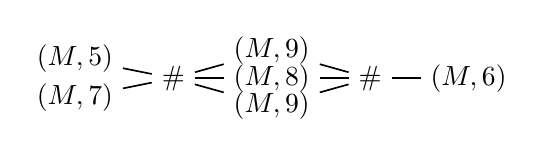
\begin{tikzpicture}[-, >=to, auto, node distance=1.25cm, semithick, transform shape]
\node (M1) {};
\node (T1) [above of=M1, node distance=0.25cm] {$(\tg M,5)$};
\node (B1) [below of=M1, node distance=0.25cm] {$(\tg M,7)$};
\node (M2) [right of=M1] {$\tg\#$};
\node (M3) [right of=M2] {$(\tg M,8)$};
\node (T3) [above of=M3, node distance=0.35cm] {$(\tg M,9)$};
\node (B3) [below of=M3, node distance=0.35cm] {$(\tg M,9)$};
\node (M4) [right of=M3] {$\tg\#$};
\node (M5) [right of=M4] {$(\tg M,6)$};
%
\path (T1) edge (M2);
\path (B1) edge (M2);
\path (M2) edge (T3);
\path (M2) edge (M3);
\path (M2) edge (B3);
\path (T3) edge (M4);
\path (M3) edge (M4);
\path (B3) edge (M4);
\path (M4) edge (M5);
\end{tikzpicture}
}%
\vspace{-1ex}
\newline
where a line from left to right indicates that the item on the right must occur after the item on the left. The end-of-second markers $\tg\#$ separate multisets of natural numbers. So, the set of data traces of $X$ has an isomorphic representation as the set $\text{Bag}(\mathbb{N})^+$ of nonempty sequences of multisets of natural numbers. In particular, the empty sequence $\epsilon$ is represented as $\emptyset$ and the single-element sequence $\tg\#$ is represented as $\emptyset \; \emptyset$.
\end{example}

Key properties described in the data trace types work bear close resemblance to the properties in \Cref{sec:operator-properties}.
The notion of a \emph{data-string transduction} is similar to a monotone operator; it is a monotone function $f: A^* \to B^*$. (So to be precise, a data-string transduction is a monotone functional operator.)
Going further, the definition of \emph{consistency}, which describes when a data-string transduction gives rise to a data-trace type, bears close resemblance to type safety and determinism of operators:

\begin{definition}[Consistency]
Let $X = (A,D)$ and $Y = (B,E)$ be data-trace types. We say that a data-string transduction $f: A^* \to B^*$
is \emph{$(X,Y)$-consistent} if $u \equiv_D v$ implies that $\bar{f}(u) \equiv_{E} \bar{f}(v)$ for all $u, v \in A^*$.
\end{definition}
